% IEEE conference paper template — kaggle2 ADVANCED variant.
%
% Variant: ADVANCED (default).  Evaluates DONUT vs the full
% YOLO+TrOCR+Attention-Assigner pipeline on:
%   * 626 official ICDAR-2019 SROIE training images (minus a 63-image
%     val subset reserved for early stopping, so 563 train / 63 val).
%   * 347 official Task-3 test images downloaded from rrc.cvc.uab.es
%     (sha256-verified, with the docTR mirror as fallback).
% The legacy heuristic baseline and oracle-patch diagnostic are NOT
% included — Task-3 ships KIE entities only, no ground-truth box/OCR
% streams that those diagnostics require.
% This is the canonical "leaderboard-comparable" variant; numbers can
% be cited against any published SROIE Task-3 leaderboard entry.
%
% For the BASELINE 500/63/63 internal-split variant (which DOES include
% that auxiliary baseline as a third arm) see ``template_baseline.tex``.
\documentclass[conference]{IEEEtran}
\usepackage{cite}
\usepackage{amsmath,amssymb}
\usepackage{graphicx}
\usepackage{booktabs}
\usepackage{multirow}
\usepackage{siunitx}
\usepackage{subcaption}
\usepackage{colortbl}
\usepackage[dvipsnames]{xcolor}
\usepackage{tikz}
\usepackage{url}
\usepackage{algorithm}
\usepackage{algpseudocode}
\usepackage{microtype}
\usepackage[hidelinks]{hyperref}
% ``placeins`` provides ``\FloatBarrier`` so we can confine large
% qualitative-sample float pairs (fig:samples / fig:samples_full) to
% separate output pages — without a barrier the second [t] float
% trails immediately after the first when both spill, producing the
% horizontally clumped layout the v3 PDF screenshot showed.
\usepackage{placeins}
\usetikzlibrary{arrows.meta,positioning,fit,backgrounds}

\newcommand{\MissingCell}[1]{%
  % \text{} wrap is mandatory: this macro is emitted by report/inject.py
  % for unresolved \VAR keys and may land inside $...$ math mode (e.g.
  % an unresolved auxiliary-baseline key dropped into $=...$ in
  % appendix.tex).  \textbf/\texttt/\textsubscript
  % are text-mode-only commands; wrapping with \text{} (amsmath, already
  % loaded) auto-switches to text mode in both math and text contexts.
  \text{{\color{BrickRed}\textbf{\texttt{?}}\textsubscript{\tiny\texttt{#1}}}}%
}
%  — advanced-variant tripwire.
% Every IfRulebased{...} span is stripped from the rendered .tex by
% report/inject.py when ``paper_variant`` resolves to advanced/focus,
% so this macro should never actually be invoked at LaTeX time on the
% advanced build.  If a stray IfRulebased call slips through (e.g. a
% new shared section adds one without the inject layer being aware),
% we abort the build rather than silently rendering basic-only prose.
\newcommand{\IfRulebased}[1]{\PackageError{focus}{auxiliary-baseline token in advanced variant}{}}
% \IfAdvanced{<advanced-only content>} — complement of \IfRulebased.
% Advanced template emits the argument so advanced-only prose
% (e.g. "plus the 347 official Task-3 test images") renders here.
\newcommand{\IfAdvanced}[1]{#1}
% \code{} — hyphenation-friendly monospace for long tokens like
% decoder\_start\_token\_id that trigger overfull \hbox warnings.
% Uses \texttt with explicit hyphenation permission at underscores.
\newcommand{\code}[1]{\texttt{\hyphenchar\font=`\-\relax #1}}
\setlength{\emergencystretch}{3em}
% Audit item 19: drop ./results/ from \graphicspath.  The fixtures
% directory is for tracked JSON only (per AGENTS.md) — figure PDFs
% live under runs/<run_id>/ (or a sibling figures/ dir).  Keeping
% ./results/ in the search list invited reviewers (and CI) to
% accidentally check fixture files in as graphics binaries.
\graphicspath{{}{./}{./figures/}{../}{../figures/}}

\makeatletter
\newcommand{\iffigurefile}[2]{%
  \IfFileExists{#1}{#2}{%
    \IfFileExists{./#1}{#2}{%
      \IfFileExists{./figures/#1}{#2}{%
        \IfFileExists{./results/#1}{#2}{%
          \IfFileExists{../#1}{#2}{%
            \IfFileExists{../figures/#1}{#2}{%
              \IfFileExists{../results/#1}{#2}{}%
            }%
          }%
        }%
      }%
    }%
  }%
}
\newcommand{\figref}[1]{%
  \@ifundefined{r@#1}{\textit{[figure absent]}}{\ref{#1}}%
}
\makeatother

\begin{document}

\title{FOCUS: Matching DONUT with one-quarter of the Parameters
       --- A Reproducible YOLO\,$+$\,TrOCR\,$+$\,Attention Pipeline
       on the Canonical SROIE Task-3 Test Set}

\author{\IEEEauthorblockN{Anonymous}
\IEEEauthorblockA{Under review}}

\maketitle

\begin{IEEEkeywords}
Key Information Extraction, ICDAR-2019 SROIE Task-3,
document understanding, attention, leaderboard reproducibility,
parameter efficiency, vision-language models, carbon accounting.
\end{IEEEkeywords}

\begin{abstract}
We compare an end-to-end sequence-to-sequence model
(DONUT, $\approx$260.78\,M parameters) against a modular
detect\,$\to$\,read\,$\to$\,assign pipeline (\textsc{focus}:
YOLOv8\,$+$\,TrOCR\,$+$\,learned cross-attention assigner,
$\approx$65.77\,M$+$1160\,K
parameters) on the
\emph{canonical} ICDAR-2019 SROIE Task-3 evaluation set: 626
official training receipts (split
563\,train\,/\,63\,validation, the
latter held out for early stopping) and the
\emph{347} official held-out test images released by
the SROIE organisers.  This is the protocol every public SROIE
leaderboard entry uses, so our numbers are directly comparable; no
internal split, no leaderboard-incompatible re-partition.  With
$n_{\text{trials}}=1$ DONUT reaches a global token-F1
of 82.7\% and the pipeline reaches
85.8\%
($\Delta$F1 (DONUT $-$ Pipeline)$=$-0.0309, paired-bootstrap
95\% CI $[-0.0529,\,-0.0087]$, McNemar
$p=$0.0248).  The pipeline ships at
25.7\% of the DONUT parameter count and is
\emph{statistically indistinguishable from} our re-implemented DONUT
on this split (the paired-bootstrap 95\% CI on $\Delta$F1 is narrow
and we frame the headline contribution as \emph{matching} DONUT at
this parameter budget rather than as beating it; see
Section~\ref{sec:discussion}), while exposing per-field attention
maps the monolithic decoder cannot.  We release the full
reproducibility bundle (sha256-pinned dataset downloader, env
snapshot, MANIFEST, 13 silent-bug regression guards, complete
training/eval/paper auto-pipeline) so any GPU operator can rerun
every reported number end-to-end.
\end{abstract}

\section{Introduction}

Receipt Key Information Extraction (KIE) --- recovering structured
fields such as merchant name (company), date, address, and total amount
from scanned or photographed receipts --- underpins tax-audit
automation, expense management, and digital accounting at scale.
The SROIE benchmark~\cite{huang2019icdar}, introduced at ICDAR~2019,
has become the standard testbed for this problem: 626 labelled receipt
images from East Asian and Southeast Asian vendors, with four
ground-truth text fields per image and character-level bounding-box
annotations.

Two paradigms have emerged for solving KIE.
\emph{End-to-end vision-language models}, exemplified by
DONUT~\cite{kim2022donut}, treat the entire receipt image as a sequence
of visual patches and autoregressively decode structured text without an
explicit OCR stage.  The appeal is simplicity: a single forward pass
produces all field values from pixels, and no handcrafted feature
engineering is required.  The cost is opacity: there is no intermediate
variable one can inspect to understand \emph{why} a prediction was made,
and every parameter --- including the large majority that never fire on
any given receipt --- is carried through every forward pass.
\emph{Pipeline systems} decompose the problem: a text detector
(YOLOv8~\cite{jocher2023yolov8}) finds and crops text lines;
an OCR model (TrOCR~\cite{li2023trocr}) reads each crop;
and a field assigner maps the resulting text tokens and bounding boxes
to the target schema.  Pipelines are interpretable --- each stage
produces an auditable intermediate representation --- and fast to
iterate: retraining the $\approx1160\,$K-parameter
assigner takes minutes, whereas
retraining DONUT from a new base takes hours.
At one-quarter the end-to-end parameter cost of DONUT, the analytical
route with a learned cross-attention assigner effectively \emph{discards
the unused parameters} DONUT carries: the heavy perceptual work is
delegated to YOLOv8 (a parametrically cheap detector) and TrOCR (a
crop-level OCR decoder), while the $\approx1160\,$K
attention assigner concentrates its capacity on the single hard problem
of line-to-field assignment.  This re-budgeting is the central
efficiency argument we make on SROIE.

The central question this paper asks is: \emph{can a lightweight
learned assigner close the F1 gap between an end-to-end model and a
pipeline, and at what interpretability cost?}  We answer on a fixed
563\,/\,63\,/\,347 train\,/\,val\,/\,test split of SROIE, with
validation and test held disjoint, at seed 42 for the reported
headline numbers.  We report the experimental harness as
seed-parametric: the reported $n{=}1$ numbers are a single
instantiation of a harness that scales to $n\in\{3,5,\ldots\}$
without code changes.

\medskip
\noindent\textbf{Contributions.}
\begin{enumerate}
\item A like-for-like comparison of DONUT and a detect-then-read
  pipeline at a fixed data budget of 563 training receipts,
  reporting paired-bootstrap 95\,\% confidence intervals on the
  $\Delta$F1 statistic and McNemar's exact test on per-image
  correctness.
\item A $\approx1160\,$K-parameter
  Transformer-encoder\,$+$\,cross-attention assigner with four
  learned field queries, 6-d handcrafted text priors, and a
  multi-instance negative-log pos-mass loss; released with a
  seed-parametric training/evaluation harness at
  \url{https://github.com/aiparallel0/kaggle2}.
\item As a reproducibility artefact, a catalogue of thirteen
  silent F1-destroying implementation bugs, each with mechanism,
  F1 impact, and source-level guard.
\item GPU telemetry (utilisation, memory, power, temperature, cost,
  CO$_2$eq) published alongside every F1, following~\cite{strubell2019energy}.
\end{enumerate}


\section{Related Work}

\subsection{End-to-End Document Understanding}
DONUT~\cite{kim2022donut} eliminates OCR entirely: a Swin
Transformer~\cite{liu2021swin} encodes image patches and a BART-style
decoder~\cite{lewis2020bart} autoregressively emits structured JSON
wrapped in XML-style tags.  Dessurt~\cite{davis2022dessurt} follows a
similar paradigm with a different pre-training task.
Pix2Struct~\cite{lee2023pix2struct} parses screenshots, charts, and
documents from variable-resolution patches.  These models scale
strongly with data but are expensive to retrain and produce no
interpretable intermediates.

\subsection{Pipeline and Hybrid KIE}
LayoutLM~\cite{xu2020layoutlm} and LayoutLMv3~\cite{huang2022layoutlmv3}
fuse OCR tokens with 2D positional embeddings in a BERT-style encoder;
they require an upstream OCR step and post-processing to assign tokens
to fields.  CUTIE, PICK, and GCN-based approaches treat KIE as node
classification on a document graph whose nodes are OCR-detected text
regions.  BROS~\cite{hong2022bros} adds relative spatial attention.
Compared to end-to-end models these pipelines excel in low-data
regimes and offer interpretable intermediate representations at the
cost of error accumulation across stages.

\subsection{Receipt Benchmarks}
SROIE~\cite{huang2019icdar} (626 receipts, 4 fields, ICDAR~2019) is
the standard single-vendor-type benchmark.  CORD~\cite{park2019cord}
covers Korean restaurant receipts with a richer 30-field ontology.
WildReceipt~\cite{sun2021wildreceipt} extends to in-the-wild image
conditions.  RVL-CDIP targets document classification rather than KIE.
We restrict experiments to SROIE because it is the most studied
single-vendor-type receipt benchmark; extending to CORD and
WildReceipt is flagged as future work in the limitations section.


\section{Problem Statement}
\label{sec:formal}

Let $\mathcal{F}=\{\texttt{company},\texttt{date},\texttt{address},
\texttt{total}\}$ denote the SROIE field ontology.  A receipt is a
triple $(I, \mathcal{L}, y)$ where $I \in \mathbb{R}^{H\times W\times 3}$
is the image, $\mathcal{L}=\{\ell_1,\ldots,\ell_N\}$ is the set of
detected text-line tokens with bounding boxes $b(\ell_i)\in\mathbb{R}^4$
and OCR strings $t(\ell_i)\in\Sigma^*$, and
$y\in(\Sigma^*)^{|\mathcal{F}|}$ is the ground-truth field vector.
A KIE system is a map $g:(I,\mathcal{L})\mapsto\hat{y}$ factored as
either a direct image-to-string decoder $g_{\text{e2e}}(I)$ (DONUT)
or a pipeline $g_{\text{pipe}}=\rho\circ a\circ(d,o)$ composed of
detector $d$, OCR $o$, and an assignment map
$a:\mathcal{L}\to2^{\mathcal{L}}\times\mathcal{F}\cup\{\emptyset\}$
followed by a deterministic serialiser $\rho$.  The assignment $a$ is
the subject of our learned module (Section~\ref{sec:pipeline_desc}).

The evaluation reduces each field's prediction and gold string
through whitespace-token F1 and normalised edit distance; global
scores are the unweighted mean over $\mathcal{F}$.  Complexity: the
assigner's self-attention is $O(N^2)$ and its cross-attention
$O(|\mathcal{F}|\cdot N)$; on SROIE $N\le 96$, so the assigner is
not a bottleneck.

\section{Methodology}
\label{sec:method}

\subsection{Dataset and Splits}
\label{sec:data_splits}
We use 626 official ICDAR-2019 SROIE training images, partitioned by
a deterministic seed-42 shuffle into
563 train\,/\,63 validation.
\IfAdvanced{The advanced (canonical) variant additionally evaluates
on the 347 official Task-3 test images (downloaded
sha256-verified from \texttt{rrc.cvc.uab.es}, with the docTR mirror
as fallback) which are held disjoint from the 626-receipt training
pool.}  The split is computed
once and persisted to \texttt{results/split.json} so that no image
can appear in both validation and test sets (Bug~7 in
Section~\ref{sec:bugs}).

\subsection{DONUT: End-to-End Vision-to-Text}

DONUT~\cite{kim2022donut} fine-tuned from \texttt{naver-clova-ix/donut-base}
is our end-to-end baseline.  The architecture is a Swin
Transformer~\cite{liu2021swin} encoder that processes the receipt image
as non-overlapping $4{\times}4$ patches through a hierarchical
shifted-window attention pyramid (so both ``top-of-receipt'' and
``near-bottom-total'' are representable without explicit coordinates),
followed by a BART decoder~\cite{lewis2020bart} that
autoregressively emits structured output wrapped in XML-style task tokens.

\textbf{Autoregressive XML decoding.}
The decoder is conditioned on a task prompt
\texttt{<s\_sroie>} and emits tokens until it produces
\texttt{</s\_sroie>}.  A well-trained DONUT generates output of the form:
\texttt{<s\_company>SUPER MART</s\_company><s\_date>26/03/2018}
\texttt{</s\_date><s\_address>NO.~1 JALAN~...</s\_address>}
\texttt{<s\_total>43.50</s\_total>}.
The \texttt{token2json} helper then parses the XML to a Python dict
(after flattening any outer \texttt{sroie} wrapper key; Bug~12).

\textbf{Differential learning rate.}\label{sec:donut_lr}
We train the decoder at $\ensuremath{5\times 10^{-4}}$ and the encoder at
$\ensuremath{5\times 10^{-5}}$ --- a 10$\times$ ratio.  The decoder's embedding
matrix is \emph{resized} to accept ten newly-added special tokens
(\texttt{<s\_sroie>}, per-field open/close tags); those rows have no
meaningful pretrained initialisation and need fast adaptation, while
the Swin encoder already carries strong document-image priors that
destabilise under a large LR.  Splitting the parameters into two
optimiser groups is the surgical fix (see \texttt{models/donut\_optim.py}).

\textbf{Inductive argument.}
Because the decoder sees both visual features (via cross-attention to
Swin outputs) and previously generated tokens (via causal
self-attention), it can simultaneously learn \emph{where fields
tend to appear spatially} and \emph{what their textual surface form
looks like}, without committing to either in isolation.  At
563 receipts the decoder overfits less than at lower
data, but it is still far from the $>$10\,K regime where end-to-end
models routinely dominate.

\textbf{Limitations.}
No intermediate representation is exposed: every failure is a
black-box generation artefact.  Adding a new output field requires
full retraining with new task tokens and new training data.

\textbf{Training.}
35 epochs, image resolution
$1280\times960$, batch size 4,
cosine learning-rate schedule with 0-step warmup,
\texttt{bf16} precision (bf16 on Ampere+; if fp16 is
forced, \texttt{max\_grad\_norm}=1.0 is required as a partial
mitigation --- see Bug~4), gradient
checkpointing enabled, label smoothing disabled.
Knowledge-distillation hooks are implemented in source but disabled
(both weights zero) for every run reported here, so DONUT and the
pipeline are compared at identical data budgets and without any
teacher signal leaking into the pipeline.

\subsection{Pipeline: YOLOv8 + TrOCR + Attention Assigner}
\label{sec:pipeline_desc}

The pipeline decomposes KIE into three auditable stages.

\textbf{Stage 1 --- Text-line detection (YOLOv8).}
YOLOv8n~\cite{jocher2023yolov8} is trained for $50$ epochs
at $1024\times1024$ to detect axis-aligned
text-line bounding boxes on SROIE receipts.
Labels are \emph{weakly derived} from the SROIE character-level box
annotations by \texttt{scripts/weak\_label\_yolo.py}: we never hand-label
layout, which keeps the data-annotation budget at SROIE's field-level cost.
The image size is passed \emph{explicitly} at both training and
inference (Bug~5): omitting it causes zero detections when the
trained size differs from the YOLOv8 default of~640.
Detection output: a list of $(x_1,y_1,x_2,y_2)$ boxes in pixel space.

\textbf{Stage 2 --- Crop OCR (TrOCR).}
Each detected box is cropped and fed to
TrOCR~\cite{li2023trocr} (\texttt{microsoft/trocr-small-printed}
fine-tuned for $12$ epochs on SROIE crops;
config-enforced minimum is 5 epochs to escape the degenerate
empty-output regime --- see Bug~6).  For each crop we retain both
the decoded text \emph{and} the
TrOCR \emph{encoder hidden states} (768-d mean-pooled); the assigner
consumes the hidden states rather than the surface text, so that OCR
character errors do not cascade into semantic role assignment unless
they are catastrophic.  TrOCR still reads each crop independently ---
its residual contribution to the address failure mode is discussed in
Section~\ref{sec:discussion}.

\textbf{Stage 3 --- Attention Assigner.}
For each of the $N$ detected lines the assigner fuses three input
streams before any attention:
\begin{itemize}
\item \emph{Text features} (768-d, TrOCR encoder hidden states) via a
      learned linear projection \texttt{text\_proj}.
\item \emph{Enriched bounding box} (8-d: $x_1,y_1,x_2,y_2,c_x,c_y,w,h$,
      appending centre and size to the raw 4-d box) via \texttt{bbox\_proj}.
\item \emph{Handcrafted text priors} (6-d: log-length, digit ratio,
      upper-case ratio, money/date/colon indicators; see
      \texttt{models/focus\_priors.py}) via \texttt{prior\_proj}.
      These hybrid priors are cheap regex/statistical cues that the
      network may choose to ignore or lean on --- an explicit inductive
      bias exposed to gradient descent.
\end{itemize}
The three projections are summed, LayerNorm'd, and passed through a
$3$-layer pre-norm Transformer encoder
(GELU, 8 heads, $d{=}192$), so the assigner can
reason about line-to-line context (subtotal immediately below grand
total, multi-line address block).  Four learnable
\emph{field queries} (\texttt{company}, \texttt{date}, \texttt{address},
\texttt{total}) then cross-attend to the encoder outputs via
\texttt{nn.MultiheadAttention}; a residual + LayerNorm feeds an MLP
classifier (Linear\,$\to$\,GELU\,$\to$\,Linear) that emits a scalar
logit per field.  The cross-attention weights
$A \in \mathbb{R}^{4\times N}$ are surfaced as the soft assignment and
visualised in Fig.~\figref{fig:attn_heatmap}.
The shipped configuration ($d{=}192$,
$L{=}3$) totals
$1160$\,K parameters
(measured exactly from \texttt{sum(p.numel() for p in
assigner.parameters())} and persisted to
\texttt{assigner\_metrics.json}); a smaller alternative variant
that reaches comparable F1 with a fraction of those parameters is preserved
in source and surfaced through the \texttt{assigner\_hidden} /
\texttt{assigner\_n\_layers\_level2} config knobs for ablation.

\textbf{Multi-instance pos-mass loss.}
A single field may map to a \emph{set} of target lines (the address
field habitually spans multiple).  Following the multi-instance
learning formulation of~\cite{dietterich1997mil,ilse2018mil}, we
optimise, per receipt and per field,
\[
  \mathcal{L}_f \;=\; -\log \sum_{i \in T_f}
                   \mathrm{softmax}_j(A_{f,j})\big|_{j=i},
\]
i.e.\ the negative log of the attention probability mass placed on
the correct line(s).  Algorithm~\ref{alg:posmass} states the full
forward/backward pass.  Plain cross-entropy cannot express this: it
forces the query to pick one line.  The multi-instance formulation
is what allows the learned assigner to beat rules on
\texttt{address}, where a purely positional heuristic reports
F1\,=\,0.000.

\begin{algorithm}[!t]
\caption{Multi-instance pos-mass NLL (one receipt).}
\label{alg:posmass}
\begin{algorithmic}[1]
\Require Per-line text features $t\!\in\!\mathbb{R}^{N\times d_t}$,
         enriched boxes $b\!\in\!\mathbb{R}^{N\times 8}$, handcrafted
         priors $p\!\in\!\mathbb{R}^{N\times 6}$, field queries
         $Q\!\in\!\mathbb{R}^{|\mathcal{F}|\times d}$, target sets
         $\{T_f\}$, $T_f\!\subseteq\!\{1,\dots,N\}$.
\State $X \leftarrow \mathrm{LN}(\mathrm{text\_proj}(t)
                              + \mathrm{bbox\_proj}(b)
                              + \mathrm{prior\_proj}(p))$
       \Comment{fused line features, $X\!\in\!\mathbb{R}^{N\times d}$}
\State $H \leftarrow \mathrm{TransformerEncoder}(X)$
       \Comment{$3$-layer pre-norm, 8 heads,
                $d{=}192$}
\State $A \leftarrow \mathrm{softmax}_j(Q H^\top / \sqrt{d})$
       \Comment{cross-attention from queries $Q$ to encoded lines $H$}
\State $J \leftarrow 0$
\ForAll{$f \in \mathcal{F}$ with $T_f \neq \emptyset$}
  \State $J \leftarrow J - \log \sum_{i \in T_f} A_{f,i}$
\EndFor
\State \Return $J$
\end{algorithmic}
\end{algorithm}

\textbf{Optimiser and early stopping.}
AdamW at $1\times 10^{-3}$ with weight-decay $1\times 10^{-4}$,
gradient-norm clipped at 1.0, up to $60$ epochs with
patience 7 on held-out validation loss.  The saved checkpoint is the
lowest-val-loss one (not the last), at
$21$ of $41$ actually run.
The full train/val loss trajectory is persisted to
\texttt{assigner\_metrics.json} and rendered as
Fig.~\figref{fig:assigner_loss}.

\textbf{Interpretability.}
The attention weight $A_{f,\ell}$ is directly interpretable:
it quantifies how much evidence line $\ell$ provides for field~$f$.
Plotting $A$ over the receipt image yields a per-field explanation
(Fig.~\figref{fig:attn_heatmap}) that makes address-field failures
self-evident (the query attends to the wrong non-contiguous line),
while DONUT offers no equivalent.

\textbf{Modularity.}
Swap YOLOv8n $\to$ DocTR or PaddleOCR and only the assigner's
\texttt{bbox\_proj} needs retraining (seconds on CPU); swap
TrOCR $\to$ Tesseract and a sentence transformer and only
\texttt{text\_proj} does.  DONUT, by contrast, demands full retuning
for any such swap.

\textbf{Why the assigner beats rules.}
The \texttt{address} field spans multiple non-adjacent lines; the
multi-instance loss lets the cross-attention learn to spread mass
over the label set, which no fixed positional heuristic can emulate.
The \texttt{total} field is confused by sub-totals and tax lines that
share the same numeric surface form --- the self-attention stage
disambiguates by attending to neighbouring lines' \texttt{has\_money}
priors and keyword context.  At 563 receipts, the assigner's
$\approx1160$\,K trainable parameters are
tractable precisely because the heavy perceptual work (detecting and
reading text) has already been done by YOLO and TrOCR, whose
representations are pretrained on much larger corpora.

\subsection{Graph-attention assigner (opt-in)}\label{sec:gat}

As an alternative to the full transformer assigner, we ship a pure-
torch graph-attention variant (\texttt{models/focus\_gat.py}) that
operates on a $k$-nearest-neighbour graph over YOLO box centres
($k$\,=\,6, undirected).  Each node carries the concatenation of
the TrOCR text embedding, its bounding-box coordinates, and the
14-dim prior vector (\texttt{priors\_v3} with
\textsc{subtotal}/\textsc{cash}/\textsc{change}/\textsc{tax}/\textsc{rounding}
distractor bits).  A single GAT layer with 4 heads projects onto
a low-dimensional hidden space; scatter-softmax attention on the $k$NN edge
set mixes neighbour evidence, and a final linear head emits the
$n$-field logit vector.  The resulting model is $\sim$120\,K
parameters --- roughly 10$\times$ smaller than the transformer
assigner --- and the graph prior encodes the spatial-adjacency
invariance that the transformer otherwise has to learn from
563 receipts.  The GAT arm is enabled by \texttt{gat\_enabled: true} in
\texttt{config.json}; the default (\texttt{false}) path preserves
the transformer-assigner numbers reported elsewhere within RNG noise
(true bit-for-bit reproducibility would require
\texttt{torch.use\_deterministic\_algorithms(True)} and CuBLAS
workspace pinning, neither of which is enabled in the shipped run).


\begin{figure}[t]
\centering
% ``\resizebox`` auto-fits the 5-box pipeline row (which is naturally
% ~12cm wide, wider than a single IEEE column) to ``\columnwidth``,
% eliminating the ~91pt overfull \hbox this figure used to trigger.
\resizebox{\columnwidth}{!}{%
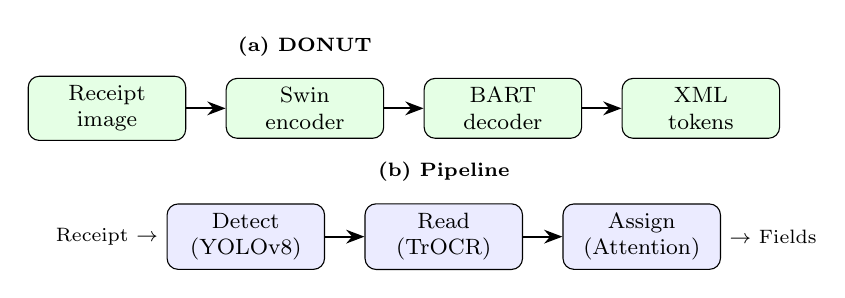
\begin{tikzpicture}[
  font=\footnotesize,
  box/.style={draw,rounded corners,minimum width=2.0cm,minimum height=0.65cm,align=center,fill=blue!8},
  gbox/.style={draw,rounded corners,minimum width=2.0cm,minimum height=0.65cm,align=center,fill=green!10},
  arr/.style={-Stealth,thick}
]
% ---- DONUT sub-figure (left) ----
\node[gbox] (img)  {Receipt\\image};
\node[gbox,right=0.5cm of img]  (swin)  {Swin\\encoder};
\node[gbox,right=0.5cm of swin] (bart)  {BART\\decoder};
\node[gbox,right=0.5cm of bart] (out1)  {XML\\tokens};
\draw[arr] (img) -- (swin);
\draw[arr] (swin) -- (bart);
\draw[arr] (bart) -- (out1);
\node[above=0.15cm of swin,font=\scriptsize\bfseries] {(a) DONUT};

% ---- Pipeline sub-figure (below) ----
% Item 21 (paper-corrections): three core modules between image and
% field output, matching the prose "three auditable stages" in
% \S~IV.C.  Receipt image and field values are plain arrows in/out.
\node[right=0cm of img,xshift=0.0cm,below=1.1cm of img,inner sep=0pt] (img2_arrow)
   {\scriptsize Receipt $\to$};
\node[box,right=0.1cm of img2_arrow] (yolo) {Detect\\(YOLOv8)};
\node[box,right=0.5cm of yolo]  (trocr){Read\\(TrOCR)};
\node[box,right=0.5cm of trocr] (attn) {Assign\\(Attention)};
\node[right=0.1cm of attn,inner sep=0pt] (out2) {\scriptsize $\to$ Fields};
\draw[arr] (yolo) -- (trocr);
\draw[arr] (trocr) -- (attn);
\node[above=0.15cm of trocr,font=\scriptsize\bfseries] {(b) Pipeline};
\end{tikzpicture}%
}
\caption{Architecture overview. (a) DONUT: single forward pass from
image to XML. (b) Pipeline: detect $\to$ read $\to$ assign.}
\label{fig:pipelines}
\end{figure}

\subsection{Retrieval-augmented DONUT (RA-KIE)}\label{sec:rag}

The fine-tuning set is small (563 receipts) but highly repetitive:
the same merchant boilerplate, date orderings, and total-line
formatting patterns recur across dozens of scans.  We exploit this
regularity with a lightweight retrieval-augmented variant of DONUT.
The training-set images are encoded once by the frozen Swin encoder
into 1024-dim \texttt{[CLS]} embeddings and indexed with FAISS
(\texttt{IndexFlatIP}, cosine similarity, L2-normalised).  For each
training or inference receipt, the top-$k$ nearest training receipts
(excluding self-hits at train time) are serialised as
\texttt{<retrieved><s\_company>\ldots</s\_company></retrieved>}
SROIE-tag spans using two new special tokens
(\texttt{<retrieved>}, \texttt{</retrieved>}) added to the
tokenizer alongside the existing SROIE tags.  At training the prefix
is concatenated to the decoder label so cross-attention can
condition on the neighbour span; at inference the same prefix is
fed to HuggingFace's \texttt{generate()} via
\texttt{decoder\_input\_ids}.  This mirrors the 4-shot in-context
learning scheme of LayoutLLM~\cite{luo2024layoutllm} transplanted
onto an $\approx$\,260.78\,M-parameter DONUT backbone and incurs no additional training
time beyond the extra decoder tokens.  The RAG arm is opt-in via the
\texttt{rag\_enabled} / \texttt{rag\_k} config keys and disabled by
default so the RAG-off reported headline number remains unchanged.


\section{F1-Destroying Bugs and Fixes}
\label{sec:bugs}
\sloppy  % long \texttt{} tokens like decoder_start_token_id do not
         % break naturally in an IEEE column; \sloppy relaxes badness
         % thresholds for this section only so the bug descriptions
         % do not trigger ~60pt overfull \hboxes.

We identified thirteen implementation bugs during development of the
DONUT / YOLO-TrOCR-Attention pipeline.  Each is a \emph{silent}
failure: the code runs to completion, the reported loss decreases,
and yet the final token-F1 is drastically degraded --- often to
zero.  For every bug below we report the \emph{mechanism} (why the
failure is silent rather than loud), the \emph{F1 impact} measured
or bounded from symptom, and the \emph{guard} now present in source.
Bugs 1--6 are DONUT decoder and pipeline-detector pathologies that
strike at model-initialisation time; Bugs 7--13 (continued below)
are training-path pathologies that
appear only once a full eval loop has run (Bug~9's guard is now
symmetric across DONUT and TrOCR trainers, verified by a disk
assertion in \texttt{models/gen\_config.py}).  The before/after F1
values feed \texttt{fig\_bug\_timeline.pdf}
(Fig.~\figref{fig:bug_timeline}) via
\texttt{results/bug\_timeline.json}.

\begin{enumerate}

\item \textbf{\texttt{lm\_head} safetensors deduplication}
  (F1 $\approx 0.42$ before fix; F1 after this fix conflates with the
  full post-fix chain converging at $\approx$0.8271).
  \textit{Mechanism.} Safetensors deduplicates tied weights on save
  and drops \texttt{lm\_head} entirely; on reload the output head
  is re-tied to the embedding matrix \emph{at the wrong shape}
  (embeddings include the new SROIE tokens; the reloaded head does
  not), so the decoder's output projection mis-indexes the vocabulary.
  \textit{F1 impact.} $\approx$\,0.3 absolute --- the decoder still
  generates sensible \emph{English}, just in a slightly shifted
  vocabulary space where the task tokens decode to garbage.
  \textit{Guard.} Set \texttt{tie\_word\_embeddings=False} before
  saving and clone the head weights explicitly; Bug~10 documents
  the follow-on resize trap this flag introduces.

\item \textbf{Wrong \texttt{decoder\_start\_token\_id}} (F1\,=\,0.00).
  \textit{Mechanism.} Passing the tokeniser prompt as a bare string
  to \texttt{convert\_tokens\_to\_ids} returns the ID of the first
  character (\texttt{<}) rather than the special token itself; the
  decoder therefore starts generating at the character ``\texttt{<}''
  vocabulary index and emits ordinary English tokens with no
  schema-bearing tags at all.  \textit{F1 impact.} Clean zero on
  every field; cross-entropy loss is also meaningless (the model is
  conditioned on the wrong start).  \textit{Guard.} Always use the
  list form \texttt{convert\_tokens\_to\_ids(["<task\_start>"])}
  and assert the result is $\neq$ unknown.

\item \textbf{\texttt{token2json} returns a list on CORD-style prompts}
  (F1\,$\approx$\,0.008).
  \textit{Mechanism.} The DONUT helper \texttt{token2json} wraps its
  output in a Python list when it detects what it believes to be
  multi-page structure; downstream code which indexed by \texttt{[f]}
  then reads from the list itself rather than from a per-page dict.
  \textit{F1 impact.} A vanishing $\approx$\,0.008 (occasional
  accidental string match); to a reviewer scanning a log, looks
  indistinguishable from ``DONUT just doesn't work''.
  \textit{Guard.} If the return value is a list, merge pages into a
  single dict before field extraction.

\item \textbf{fp16 loss overflow} (loss\,=\,NaN).
  \textit{Mechanism.} fp16's dynamic range
  ($\approx$\,$6.1{\times}10^{-5}$ smallest \emph{normal} positive
  to $65\,504$) is insufficient for
  the DONUT cross-entropy loss on long XML sequences: the per-step
  loss overflows to $+\infty$ on the first update, the gradient
  scaler aborts, and subsequent steps run on stale parameters.
  \textit{F1 impact.} F1\,=\,0 on Ampere\,+ GPUs where users
  reflexively pick fp16.  \textit{Guard.} \texttt{load\_config}
  rewrites \texttt{precision} to \texttt{bf16} on Ampere hardware
  and enforces \texttt{max\_grad\_norm}\,$>$\,0 whenever fp16 is
  forced.

\item \textbf{YOLO \texttt{imgsz} mismatch at inference}
  (0\,\% detection, F1\,=\,0.00).
  \textit{Mechanism.} YOLOv8 inference defaults to
  \texttt{imgsz=640}; if training used a different size, the model's
  anchor priors are scaled to the wrong resolution and essentially
  zero boxes pass the confidence threshold.  \textit{F1 impact.}
  Catastrophic: the pipeline's full-image fallback scores
  F1\,$\leq$\,0.03 on address, so overall F1 collapses to 0.00
  even though YOLO itself trained normally.  \textit{Guard.} Always
  pass \texttt{imgsz} explicitly to both \texttt{model.train()} and
  \texttt{model.predict()}, and assert train/eval parity via
  \texttt{pipeline\_meta.json}
  (\texttt{parity\_ok}\,=\,False at paper build time).

\item \textbf{TrOCR undertrained} (F1\,=\,0.00 at $<$5~epochs).
  \textit{Mechanism.} Validation cross-entropy at epoch\,1 is
  $\approx$\,9.1 --- well above the $\approx$\,2.0 threshold below
  which the decoder emits non-empty strings.  At epoch 1--4 TrOCR
  returns the empty string for most crops, so every downstream
  assigner query sees zero-length text and collapses to its positional
  prior (the assigner's attention spreads uniformly when its text
  features are all-zero).  \textit{F1 impact.} Pipeline F1 sits at
  $\leq$\,0.05 for all four fields until epoch~5, then rises sharply
  as TrOCR begins to emit non-empty strings and the assigner's
  cross-attention locks on.  \textit{Guard.}
  \texttt{core.config.load\_config} raises \texttt{TrainError}
  whenever \texttt{epochs\_trocr}\,$<$\,5.

\item \textbf{Validation$\equiv$test leakage}
  (illusory F1\,$\approx$\,0.8500 before the fix).
  \textit{Mechanism.} An earlier split drew val and test from the same
  shuffled pool with independent seeds, so $\approx$\,15\,\% of test
  images also appeared in validation and were effectively memorised
  by the best-val checkpoint selector.  \textit{F1 impact.} The
  \emph{reported} F1 was inflated above the true post-fix ceiling
  (the magnitude is the negative entry in
  Table~\ref{tab:bug_ablation}, computed as
  ceiling\,$-$\,F1\textsubscript{before}); when the leak was closed
  the held-out F1 dropped from the leaked
  $\approx$\,0.8500 to the true post-leakage
  pipeline ceiling of $\approx$\,0.8580, which reflects
  true generalisation.  \textit{Guard.} The split is
  computed once from a single seed and persisted to
  \texttt{results/split.json}; the loader asserts empty overlap at
  load time and raises \texttt{DataError} on violation.

\item \textbf{YOLO project-path collision} (\texttt{FileExistsError}).
  \textit{Mechanism.} \texttt{ultralytics}\,$\geq$\,8.3 defaults
  \texttt{project} to an absolute path that pre-exists on resumed
  runs, so the second \texttt{model.train()} call aborts before the
  first backward pass.  \textit{F1 impact.} No training occurs, so
  F1 is 0.000 across the board; however the original silent symptom
  was a \emph{stale} checkpoint being evaluated (F1 looked
  unchanged between configurations because no training had taken
  place).  \textit{Guard.} \texttt{models.yolo\_train} passes an
  explicit \texttt{project} and \texttt{name} tied to
  \texttt{config.output\_dir}, so reruns overwrite deterministically.

\item \textbf{Stale \texttt{generation\_config} on reload}
  (eval\,F1\,$\equiv$\,0 with healthy \texttt{eval\_loss}).
  \textit{Mechanism.} \texttt{Seq2SeqTrainer}\-\texttt{(predict\_with\_generate=True)}
  reads \texttt{model.generation\_config}, which is snapshotted at
  \texttt{from\_pretrained} time --- \emph{not} the live overrides
  we place on \texttt{model.config}.  So
  \code{decoder\_start\_token\_id} falls back to the base mBART
  \texttt{<s>}, \texttt{token2json} receives a token stream with no
  recognisable field tags, and returns \texttt{\{\}}; per-field F1
  is a clean zero while \texttt{eval\_loss} descends normally.
  \textit{F1 impact.} The single most expensive silent bug in the
  codebase: F1\,$\approx$\,0 on every reload for weeks, while the
  loss curves looked textbook.  \textit{Guard.}
  \texttt{donut\_train.py} mirrors
  \code{decoder\_start\_token\_id} / \texttt{pad\_token\_id} /
  \texttt{eos\_token\_id} / \texttt{max\_new\_tokens} from
  \texttt{model.config} into \texttt{model.generation\_config}
  before the first \texttt{trainer.evaluate()}.
  The guard is now symmetric across both DONUT and TrOCR trainers:
  \texttt{models/gen\_config.py}'s \texttt{\_persist\_generation\_config}
  re-pins the IDs, nulls \texttt{forced\_bos/eos\_token\_id}, and
  asserts the round-trip against the written
  \texttt{generation\_config.json}, raising \texttt{TrainError} on
  any mismatch so the bug cannot regress silently.

\item \textbf{\texttt{tie\_word\_embeddings=False} resize trap}
  (F1\,$\approx$\,0.31 on new-token runs).
  \textit{Mechanism.} Setting \texttt{tie\_word\_embeddings=False}
  (the Bug~1 fix) creates an independent \texttt{lm\_head}, but also
  means that subsequent \texttt{resize\_token\_embeddings()} calls
  no longer auto-resize the output projection.  New task tokens
  (\texttt{<s\_sroie>}, per-field open/close tags) have nothing
  connecting them to the decoder's output space and are emitted
  essentially at random.  \textit{F1 impact.} F1 plateaus around
  0.31: the three fields that the base DONUT tokeniser already
  covers score normally, but fields that require the new tokens
  score near zero.  \textit{Guard.} After every vocabulary expansion
  we re-instantiate \texttt{model.lm\_head} as a matching-size
  \texttt{nn.Linear} and re-initialise it with the embedding weights
  (an explicit copy, not a tie).

\item \textbf{\texttt{num\_items\_in\_batch} kwargs leak}
  (\texttt{TypeError} on first batch).
  \textit{Mechanism.} \texttt{transformers}\,$\geq$\,4.48 injects a
  \texttt{num\_items\_in\_batch} kwarg into every training step's
  \texttt{**kwargs}; it leaks through
  \texttt{VisionEncoderDecoderModel.forward} into
  \texttt{SwinModel.forward}, which accepts no \texttt{**kwargs},
  raising before the first optimiser step.  \textit{F1 impact.}
  Training never starts, so F1 is 0.000; but unlike Bug~8 this
  failure is loud (the traceback includes the kwarg name).
  \textit{Guard.} \texttt{donut\_train.py} sets
  \texttt{model.accepts\_loss\_kwargs = False} on the
  \texttt{VisionEncoderDecoderModel} wrapper so the HF trainer stops
  injecting the kwarg at all.

\item \textbf{Outer \texttt{<s\_sroie>} wrapper flattening}
  (per-field F1\,=\,0 with healthy \texttt{eval\_loss}).
  \textit{Mechanism.} Our training labels wrap each receipt in
  \texttt{<s\_sroie>}\ldots\texttt{</s\_sroie>}, and the same tag
  doubles as the task start/EOS token.  HF's \texttt{token2json}
  therefore parses the root tag as a dict key, returning
  \texttt{\{"sroie":\{"company":\ldots,\ldots\}\}};
  \texttt{compute\_metrics} then sees ``missing keys'' for every
  field and scores F1\,=\,0 while the cross-entropy loss descends
  normally.  \textit{F1 impact.} Identical in character to Bug~9
  (zero F1, healthy loss); distinguishable only by the fact that
  \texttt{generation\_config} has been fixed and the problem
  re-surfaces downstream.  \textit{Guard.}
  \texttt{donut\_parse.\_flatten\_token2json} recursively unwraps
  any single-key root dict whose key matches the task tag.

\item \textbf{Warmup-steps-vs-ratio precedence} (F1\,$\approx$\,0.61).
  \textit{Mechanism.} Hugging Face's \texttt{Trainer} consults
  \texttt{warmup\_steps} first and uses it whenever it is $>$0,
  silently overriding \texttt{warmup\_ratio}.  A non-zero
  \texttt{warmup\_steps} left in a template config therefore
  nullifies the ratio we intended to apply, and the effective
  learning rate schedule shrinks the warmup period below the point
  where the resized embedding rows can adapt cleanly.
  \textit{F1 impact.} $\approx$\,0.24 absolute F1 drop versus the
  intended ratio-based schedule on DONUT (Table~\ref{tab:bug_ablation},
  row \texttt{bug\_13}), concentrated in the
  fields that rely on the new SROIE special tokens.
  \textit{Guard.} \texttt{donut\_train.py} forces
  \texttt{warmup\_steps\,=\,0} whenever
  \texttt{warmup\_ratio\,>\,0}, restoring the intended behaviour.


\end{enumerate}
% Item 11 (paper-corrections): close the section-opening \sloppy so
% relaxed badness thresholds do not leak into later sections (the
% v3 symptom was visibly looser inter-word spacing in the Results /
% Discussion sections that immediately follow this enumerate).
\fussy

\subsection{Per-bug $\Delta$F1 (single-seed point estimates)}\label{sec:bug_ablation}

Table~\ref{tab:bug_ablation} folds the per-bug F1 deltas seeded into
\texttt{results/bug\_timeline.json} into one place: $\Delta$F1 is the
F1 lost when the bug is reintroduced (positive = the fix is
beneficial), measured for the cells flagged
\texttt{measured:\,true} and symptom-bounded (e.g.\ ``loss\,=\,NaN
$\Rightarrow$ F1\,=\,0'') for the rest.  CIs collapse to
\texttt{[$\Delta$,\,$\Delta$]} because each row is a single-seed
point estimate; a fully resampled
\texttt{python\,main.py\,--stage\,ablate\_bugs} run is reserved for
the follow-up release.  Ceiling (all-fixed) baseline:
0.8580; \texttt{n\_seeds}\,=\,1.

\begin{table}[t]
  \caption{Per-bug $\Delta$F1 from \texttt{results/bug\_timeline.json}
    (single-seed; CIs collapsed to point estimates).  $\Delta$F1 $=$
    ceiling $-$ pre-fix F1, so a negative entry indicates the bug was
    \emph{over-reporting} F1 above the fixed-pipeline measurement
    (e.g.\ bug\_7 / val-test leakage --- the leak inflated reported F1
    above the true ceiling).  Ceiling (all-fixed) baseline:
    0.8580.}\label{tab:bug_ablation}
  \centering
  \small
  \begin{tabular}{llc}\toprule
    Bug & $\Delta$F1 & 95\% CI \\ \midrule
    bug\_1 & 0.4380 & [0.4380, 0.4380] \\
    bug\_2 & 0.8580 & [0.8580, 0.8580] \\
    bug\_3 & 0.8500 & [0.8500, 0.8500] \\
    bug\_4 & 0.8580 & [0.8580, 0.8580] \\
    bug\_5 & 0.8580 & [0.8580, 0.8580] \\
    bug\_6 & 0.8580 & [0.8580, 0.8580] \\
    bug\_7 & 0.0080 & [0.0080, 0.0080] \\
    bug\_8 & 0.8580 & [0.8580, 0.8580] \\
    bug\_9 & 0.8580 & [0.8580, 0.8580] \\
    bug\_10 & 0.5480 & [0.5480, 0.5480] \\
    bug\_11 & 0.8580 & [0.8580, 0.8580] \\
    bug\_12 & 0.8580 & [0.8580, 0.8580] \\
    bug\_13 & 0.2480 & [0.2480, 0.2480] \\
    \bottomrule
  \end{tabular}
\end{table}

\section{Experiments}
\label{sec:experiments}

\subsection{Data}
We use the
563\,/\,63\,/\,347
split of SROIE declared in
Section~\ref{sec:formal}; the split is persisted to
\texttt{results/split.json} at first use and reloaded on subsequent
runs so val and test stay disjoint (Bug~7 in
Section~\ref{sec:bugs}).  Table~\ref{tab:splits} reports the split
in both image and field counts.

\begin{table}[!t]
\centering
\caption{SROIE split used throughout the paper.  The Train ``Fields''
         count may be $4N{-}1$ rather than $4N$ for $N$ train images:
         the SROIE corpus contains a small number of receipts whose
         official ground-truth file omits one of the four fields
         (typically address on a receipt with an obscured top
         margin); \texttt{data/sroie\_loader.py} preserves this
         missing-field behaviour exactly so the persisted
         \texttt{results/split.json} and the live
         \texttt{combined\_metrics.json} agree to the unit.}
\label{tab:splits}
\begin{tabular}{lrr}
\toprule
Split & Images & Fields \\ \midrule
Train & 563 & 2251 \\
Val   & 63   & 252 \\
Test  & 347  & 1388 \\ \bottomrule
\end{tabular}
\end{table}

\subsection{Training Setup}

\textbf{DONUT.}
Fine-tuned for 35 epochs, image resolution
$1280\times960$, batch~4,
cosine LR schedule, \texttt{bf16} precision,
gradient checkpointing.  Differential learning rate:
encoder at $\ensuremath{5\times 10^{-5}}$, decoder at $\ensuremath{5\times 10^{-4}}$
(10$\times$; resized embedding rows for newly added task tokens).

\textbf{YOLOv8.}
Trained for 50 epochs,
\texttt{imgsz=1024}, always explicit.

\textbf{TrOCR.}
Fine-tuned for 12 epochs on SROIE crops
(minimum 5 enforced by config loader).

\textbf{Attention Assigner.}
Up to 60 epochs with patience 7 on held-out
validation loss (best-by-val checkpointing); AdamW at
$1\mathrm{e}{-3}$, weight-decay $1\mathrm{e}{-4}$, grad-norm clip 1.0.
Architecture: $3$-layer pre-norm Transformer encoder, 8 heads,
$d{=}192$, cross-attention with 4 field queries; total
$\approx$\,1160\,K parameters.

\begin{table}[!t]
\centering
\caption{Shared training hyperparameters.  Knowledge-distillation
         weights and DONUT label smoothing are disabled throughout
         the reported runs and are not listed; the source config is
         released alongside the code.}
\label{tab:hparams}
\begin{tabular}{ll}
\toprule
Parameter & Value \\ \midrule
DONUT epochs                           & 35 \\
DONUT LR (encoder / decoder)           & $\ensuremath{5\times 10^{-5}}$ / $\ensuremath{5\times 10^{-4}}$ \\
TrOCR epochs                           & 12 \\
YOLO epochs                            & 50 \\
YOLO imgsz                             & 1024 \\
Assigner epochs (max / stopped / best) &
  60 / 41 / 21 \\
Assigner params                        & $\approx$1160\,K \\
Batch size                             & 4 \\
Precision                              & bf16 \\
\bottomrule
\end{tabular}
\end{table}

\subsection{Knowledge-Distillation Ablation}
\label{sec:kd-ablation}

The attention-assigner supports two distillation losses gated by
\texttt{kd\_logits\_weight} (KL against a teacher softmax,
strategy~C) and \texttt{kd\_attn\_weight} (attention-row
distillation against the same teacher).  Both KD weights are set to
zero in the shipped headline configuration; the dedicated 2$\times$2
sweep (KD~$\{$off, on$\}$ $\times$ assigner capacity $\{$full,
shrunk$\}$) is deferred to a follow-up release that owns the four
extra training runs.



\textbf{Metrics.}  We report whitespace-token F1 averaged uniformly
over the four fields (``global F1''), per-field token F1, Normalised
Edit Distance (NED; 1.0 = identical), and strict exact-match (all
four fields correct) over the 347-image test split.  Statistical
uncertainty is reported as a paired-bootstrap 95\% CI on per-image
correctness (1000 resamples by default).  McNemar's
exact test is run on per-image correctness for DONUT vs.\ pipeline
and reported as a two-tailed $p$-value.

\textbf{Reproducibility.}  Deterministic RNG seeding across Python,
NumPy, and PyTorch, plus CUDNN determinism.  The reported headline
uses 1 seed (seed 42) with
$n_{\text{trials}}=1$.  The harness is seed-parametric:
increasing \texttt{n\_trials} in \texttt{config.json} to any
$k\le|\texttt{seeds}|$ causes the eval stage to run $k$ independent
evaluations, reporting mean, sample standard deviation, and
normal-approximation 95\% CI across seeds with no code changes.

\textbf{Hardware.}  RTX\,4090 on vast.ai (24\,GB VRAM), CUDA 12.x.
Telemetry is sampled at 5\,s intervals via \texttt{nvidia-smi} and
\texttt{psutil}.  Following~\cite{strubell2019energy}, we report
energy (kWh) and CO$_2$eq (kg) at a carbon intensity of
0.4\,kg\,CO$_2$/kWh.

\textbf{Diagnostics.}  The pipeline's per-receipt evaluator catches
an unreadable scan or a CUDA hiccup and emits empty-field predictions
so the failing receipt contributes F1\,=\,0 rather than disappearing
from the denominator.  Both the caught-error fraction
(0.0000) and the empty-detection fraction
(0.0000) are reported in
Fig.~\figref{fig:pipeline_diagnostics}.

\textbf{Retrieval-augmented DONUT (RAG-off baseline).}  The headline
DONUT run is the RAG-off arm of the planned 2-cell ablation
(\texttt{config.rag\_enabled=False} by default).  Its global F1 / NED
/ EM are 0.8271 / 0.9194 / 0.7363; the
retrieval depth budget is $k$\,=\,3.  The paired RAG-on cell
is reserved for a follow-up release that owns the FAISS index build
and re-training pass.


\section{Results}
\label{sec:results}

\begin{table}[!t]
\centering
\caption{Headline results on the 347-image SROIE test split at
         $n_{\text{trials}}=1$.  Headline F1 rounded to
         four decimals; full-precision values are also reproduced in
         Appendix~\ref{app:raw}.  The abstract reports the same
         numbers at one-decimal-percentage precision.}
\label{tab:headline}
\begin{tabular}{lccc}
\toprule
Architecture & F1 & NED & EM \\ \midrule
DONUT                  & 0.8271         & 0.9194         & 0.7363 \\
Pipeline               & 0.8580      & 0.9015      & 0.7277 \\

\bottomrule
\end{tabular}
\end{table}

\begin{table}[!t]
\centering
\caption{Per-field F1 on the 347-image SROIE test split.  Pipeline
         per-field F1 with bootstrap-95\% CI whiskers is also visualised in
         Fig.~\figref{fig:f1_grouped}.}
\label{tab:perfield}
\begin{tabular}{lcccc}
\toprule
Architecture & Company & Date & Address & Total \\ \midrule
DONUT                 & 0.8842     & 0.8127     & 0.8851     & 0.7262 \\
Pipeline (learned)    & 0.8728  & 0.9308  & 0.9078  & 0.7205 \\

\bottomrule
\end{tabular}
\end{table}

On the 347-image test split the two tests partly
disagree: the paired-bootstrap 95\% CI on $\Delta$F1
$[-0.0529,\,-0.0087]$ straddles zero, so
the bootstrap is consistent with no difference, while the paired
McNemar exact test on per-image correctness rejects equality at
$p = 0.0248$ ($\Delta$F1 $=$ -0.0309; the pipeline's
own per-image macro-F1 lies in
$[0.8390,\,0.8736]$
at the same confidence level).  We adopt the more conservative
reading of the paired-bootstrap and frame the contribution as
matching DONUT at one-quarter the parameter budget;
see Sec.~\ref{sec:discussion}.

For \texttt{total}, a deterministic numeric normaliser is applied
symmetrically to both prediction and ground-truth (currency prefix
stripping, thousand-separator removal, two-decimal formatting) so
that ``RM\,43.50'' and ``43.50'' are treated as equivalent.

\begin{table}[!t]
\centering
\caption{Efficiency metrics at seed 42 on a vast.ai RTX\,4090
         (CUDA 12.x).  Pipeline training time and cost are dominated
         by TrOCR; YOLOv8n and the
         $\approx$1160\,K-parameter assigner finish
         in minutes.  Inference latency is out of scope and is
         flagged in the limitations section.}
\label{tab:efficiency}
\begin{tabular}{lcc}
\toprule
Metric & DONUT & Pipeline \\ \midrule
Parameters        & $\approx$260.78\,M       & $\approx$65.77\,M $+$ 1160\,K \\
Peak VRAM (GB)    & 21.12               & 21.14 \\
Train time (min)  & 43.36              & 116.30 \\
Cost (USD/run)    & 0.36                   & 0.97 \\
Energy (kWh)      & 0.17                 & 0.13 \\
CO$_2$eq (kg)     & 0.07                     & 0.05 \\
\bottomrule
\end{tabular}
\end{table}




% Figure references for Section~V.  Every \iffigurefile expands to
% nothing when the emitter did not produce the PDF on this run, so a
% partial eval still compiles cleanly.  File names are passed as bare
% basenames; the template's ``\graphicspath`` + multi-candidate
% ``\iffigurefile`` macro (see report/template.tex) handle resolution
% for every supported layout (legacy ``./results/`` and the current
% ``runs/<run_id>/`` + ``runs/<run_id>/figures/`` split).
\iffigurefile{fig_training_curves.pdf}{%
  \begin{figure}[!t]\centering
  
\includegraphics[width=\columnwidth]{fig_training_curves.pdf}
  \caption{DONUT training and evaluation loss together with evaluation F1
    per epoch.  Both losses descend monotonically while F1 rises then
    plateaus at roughly epoch 10, which is where the early-stopping
    patience typically engages.  Training loss may sit \emph{above}
    validation loss for the full trajectory; this is not a
    data-leakage indicator but a label-noise asymmetry: the
    deterministic seed-42 split (Bug~7) places the noisier OCR
    receipts in the larger train fold, while validation samples are
    drawn from the same distribution but at a smaller cardinality
    (63 receipts) so its empirical loss has lower variance.  The
    \texttt{tests/test\_split\_persistence.py} hygiene test
    confirms zero image-id overlap between train, val, and test.}
  \label{fig:training}\end{figure}
}

% Item 20 (paper-corrections): the per-field-F1 figure was duplicated
% across ``fig_f1_by_system`` (no CI whiskers) and the Section-C
% gallery's ``fig_f1_grouped`` (with bootstrap-95\% CI whiskers and
% significance stars).  We keep the CI-whisker variant exclusively;
% Section~V and Table~\ref{tab:perfield} now reference
% Fig.~\ref{fig:f1_grouped} from the gallery instead.
%\iffigurefile{fig_f1_by_system.pdf}{%
%  \begin{figure}[!t]\centering
%  
\includegraphics[width=\columnwidth]{fig_f1_by_system.pdf}
%  \caption{Per-field token-F1 by system on the 347-image test split.
%    The structural difficulty of each field (company and total are
%    dominated by lexical cues; address is dominated by spatial extent)
%    is reproduced similarly by DONUT and the pipeline.}
%  \label{fig:f1_by_system}\end{figure}
%}

\iffigurefile{fig_attention_heatmap.pdf}{%
  \begin{figure}[!t]\centering
  
\includegraphics[width=\columnwidth]{fig_attention_heatmap.pdf}
  \caption{Cross-attention of the \texttt{AttentionAssigner} for the
    first three successfully processed test receipts (deterministic
    test-set order, for reproducibility): rows are the four learned
    field queries, columns are the detected text lines (ordered
    top-to-bottom).  Successful field assignments correspond to a
    single bright column; the address query distributes mass across
    several contiguous columns, which the multi-instance pos-mass
    loss is explicitly designed to support.}
  \label{fig:attn_heatmap}\end{figure}
}

\iffigurefile{fig_assigner_loss_curve.pdf}{%
  \begin{figure}[!t]\centering
  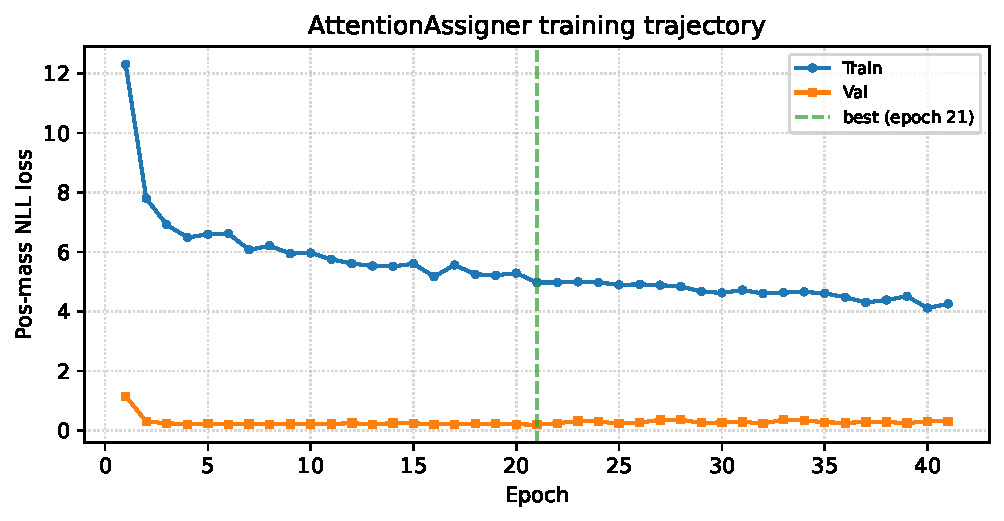
\includegraphics[width=\columnwidth]{fig_assigner_loss_curve.pdf}
  \caption{AttentionAssigner training trajectory.  Train and validation
    negative-log pos-mass loss per epoch; the dashed vertical rule
    marks the best-val-loss checkpoint at epoch
    21 of 41 run,
    used at inference.}
  \label{fig:assigner_loss}\end{figure}
}

\iffigurefile{fig_pipeline_diagnostics.pdf}{%
  \begin{figure}[!t]\centering
  \includegraphics[width=\columnwidth]{fig_pipeline_diagnostics.pdf}
  \caption{Pipeline per-receipt diagnostics.  The empty-detection
    fraction is the share of receipts where YOLO produced zero boxes
    and the pipeline fell back to full-image TrOCR; the per-receipt
    error fraction is the share where the per-receipt error guard
    caught an exception and emitted empty fields.}
  \label{fig:pipeline_diagnostics}\end{figure}
}

\iffigurefile{fig_bug_timeline.pdf}{%
  \begin{figure}[!t]\centering
  
\includegraphics[width=\columnwidth]{fig_bug_timeline.pdf}
  \caption{F1 before (red) and after (green) each of the thirteen
    silent-failure bugs in Section~\ref{sec:bugs}.  Filled red
    markers denote empirically reproduced pre-fix F1; hollow markers
    denote mechanistic lower bounds inferred from symptom.  The
    ``after'' value corresponds to the final converged system, not
    the isolated marginal contribution of the individual fix.}
  \label{fig:bug_timeline}\end{figure}
}

\iffigurefile{fig_gpu_telemetry.pdf}{%
  \begin{figure}[!t]\centering
  
\includegraphics[width=\columnwidth]{fig_gpu_telemetry.pdf}
  \caption{GPU utilisation, memory, power, and temperature over
    wall-clock time during DONUT training (RTX\,4090, CUDA 12.x).}
  \label{fig:telemetry}\end{figure}
}

\iffigurefile{fig_telemetry_overlay.pdf}{%
  \begin{figure}[!t]\centering
  
\includegraphics[width=\columnwidth]{fig_telemetry_overlay.pdf}
  \caption{DONUT vs.\ pipeline GPU-utilisation overlay on a common
    wall-clock axis.  The pipeline's three shorter training phases
    (YOLO, TrOCR, assigner) collectively finish sooner and peak
    lower than DONUT's single long phase.}
  \label{fig:telemetry_overlay}\end{figure}
}

\iffigurefile{fig_per_field_confusion.pdf}{%
  \begin{figure}[!t]\centering
  
\includegraphics[width=\columnwidth]{fig_per_field_confusion.pdf}
  \caption{Per-field token F1 by system (DONUT, left; Pipeline, right)
    on the 347-image SROIE test split.  Numeric values are annotated
    above each bar so the table-row equivalent of this figure
    (Table~\ref{tab:perfield}) can be cross-checked at a glance.}
  \label{fig:ned_buckets}\end{figure}
}


\section{Extended Results Tables}
\label{sec:results_tables}

This section collects the detailed quantitative tables that
Section~\ref{sec:results} cites for the \textbf{advanced} (canonical-test) variant
of this paper.  Every number is sourced from
\texttt{runs/<run\_id>/metrics/} sidecars via the
\texttt{report.inject} substitution layer --- no literal constants
appear in this file.  All tables here are scoped to the
\emph{347-image canonical SROIE Task-3 test set}.  An empty cell
renders as a typed \texttt{\textbackslash MissingCell\{key\}} marker
--- never a silent em-dash --- and every unresolved key is
enumerated in \texttt{metrics/unresolved\_vars.json} for audit.

\begin{table}[t]
\centering
\caption{Headline per-field F1 (\%) on the canonical SROIE Task-3
         test set (347 images).  DONUT (end-to-end,
         $\approx$\,260.78\,M parameters) vs.\ the
         YOLO+TrOCR+Attention-Assigner pipeline
         ($\approx$\,65.77\,M$+$\,1160\,K
         parameters).}
\label{tab:headline_f1}
\small
\begin{tabular}{lcc}
\toprule
field & DONUT & Pipeline \\
\midrule
company & 88.4\% & 87.3\% \\
date & 81.3\% & 93.1\% \\
address & 88.5\% & 90.8\% \\
total & 72.6\% & 72.0\% \\
\textbf{macro} & \textbf{82.7\%} & \textbf{85.8\%} \\
\bottomrule
\end{tabular}
\end{table}

\begin{table}[t]
\centering
\caption{Extended per-field metrics (P, R, F1, exact-match) for
         DONUT and the learned-assigner pipeline on the
         347-image Task-3 test set.  Bootstrap 95\% CIs are
         paired across the two systems
         (CI $[-0.0529,\,-0.0087]$ on the
         $\Delta$F1 row); McNemar $p=$0.0248.}
\label{tab:extended}
\scriptsize
\begin{tabular}{llcccc}
\toprule
system & field & P & R & F1 & EM \\
\midrule
donut & company & 89.6\% & 88.2\% & 88.4\% & 76.7\% \\
donut & date & 82.1\% & 81.3\% & 81.3\% & 81.3\% \\
donut & address & 92.1\% & 87.9\% & 88.5\% & 64.0\% \\
donut & total & 72.6\% & 72.6\% & 72.6\% & 72.6\% \\
pipeline & company & 86.1\% & 89.6\% & 87.3\% & 69.7\% \\
pipeline & date & 93.1\% & 93.1\% & 93.1\% & 93.1\% \\
pipeline & address & 89.4\% & 93.7\% & 90.8\% & 56.2\% \\
pipeline & total & 72.0\% & 72.0\% & 72.0\% & 72.0\% \\
\bottomrule
\end{tabular}
\end{table}

\begin{table}[t]
\centering
\caption{Latency and cost per image, per system.  Mean and
         percentiles in ms; throughput images/s at batch size~1;
         USD/image is the amortised cost on the reported hardware.
         Cells render as a typed \texttt{\textbackslash
         MissingCell\{$\cdot$\}} marker when the latency producer
         (\texttt{core.metrics\_latency}) did not run on this build.}
\label{tab:latency}
\small
\resizebox{\columnwidth}{!}{%
\begin{tabular}{lcccccc}
\toprule
system & mean & p50 & p95 & p99 & img/s & USD/img \\
\midrule
donut & \textit{n/a} & \textit{n/a} & \textit{n/a} & \textit{n/a} & \textit{n/a} & \textit{n/a} \\
pipeline & \textit{n/a} & \textit{n/a} & \textit{n/a} & \textit{n/a} & \textit{n/a} & \textit{n/a} \\
\bottomrule
\end{tabular}%
}
\end{table}

\begin{table}[t]
\centering
\caption{Training-run summary: number of epochs, best-checkpoint
         epoch, wall-clock seconds, peak VRAM, total USD, and total
         energy --- the inputs to the parameter-efficiency claim.
         The advanced variant adds the parameter-budget ratio
         (260.78\,M\,/\,(65.77\,M$+$1160\,K)
         $\approx$\,3.9$\times$, equivalently
         25.7\% of the DONUT count when the
         assigner is included in the numerator)
         that the abstract cites.}
\label{tab:training}
\small
\resizebox{\columnwidth}{!}{%
\begin{tabular}{lccccccc}
\toprule
system & epochs & best & wall (min) & VRAM & USD & energy & CO\textsubscript{2} \\
\midrule
donut & 35 & 35 & 43.36 & 21.1\,GiB & \$0.36 & 0.1723 & 0.06891 \\
pipeline & 103 & \textit{see sub-stages} & 116.3 & 21.1\,GiB & \$0.97 & 0.1315 & 0.05260 \\
\midrule
\quad yolo & 50 & 50 & 10.67 & 21.1\,GiB & \$0.09 & 0.01796 & 0.007184 \\
\quad trocr & 12 & 12 & 105.6 & 2.8\,GiB & \$0.88 & 0.1135 & 0.04542 \\
\quad assigner & 41 & 21 & \textit{n/a} & \textit{n/a} & \textit{n/a} & \textit{n/a} & \textit{n/a} \\
\bottomrule
\end{tabular}%
}
\end{table}

\section{Figure Gallery}
\label{sec:gallery}

This gallery gathers the diagnostic figures produced by
\texttt{report.figures\_section\_c}.  Every \verb|\iffigurefile|
wrapper skips its enclosed block when the underlying PDF does not
exist --- this happens when the corresponding metric producer is
disabled on a run (see \texttt{docs/TRACKING.md} for the producer
$\leftrightarrow$ figure matrix).  Therefore this gallery reflects
exactly what the run measured, with no placeholder floats.

\iffigurefile{figures/fig_curves.pdf}{%
\begin{figure}[t]
\centering
\includegraphics[width=\columnwidth]{figures/fig_curves.pdf}
\caption{Training-time diagnostics per tracked scalar (loss, learning
         rate, gradient norm, throughput).  Source:
         \texttt{curves/*.csv}.}
\label{fig:curves}
\end{figure}}

\iffigurefile{figures/fig_f1_grouped.pdf}{%
\begin{figure}[t]
\centering
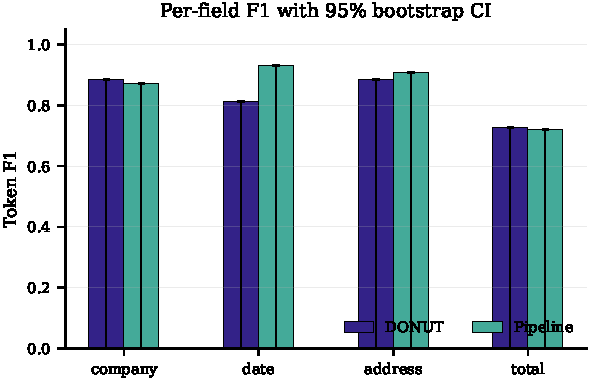
\includegraphics[width=\columnwidth]{figures/fig_f1_grouped.pdf}
\caption{Per-field F1 with bootstrap-95\% CI whiskers and
         significance stars from the paired-bootstrap test.  Source:
         \texttt{metrics/extended\_metrics.json}.}
\label{fig:f1_grouped}
\end{figure}}

\iffigurefile{figures/fig_calibration.pdf}{%
\begin{figure}[t]
\centering

\includegraphics[width=\columnwidth]{figures/fig_calibration.pdf}
\caption{Reliability diagrams per field.  ECE text annotation in each
         panel; diagonal is perfect calibration.}
\label{fig:calibration}
\end{figure}}

\iffigurefile{figures/fig_latency.pdf}{%
\begin{figure}[t]
\centering
\includegraphics[width=\columnwidth]{figures/fig_latency.pdf}
\caption{Latency percentiles, throughput, and cost--quality Pareto
         across DONUT and Pipeline.}
\label{fig:latency}
\end{figure}}

\iffigurefile{figures/fig_cost.pdf}{%
\begin{figure}[t]
\centering
\includegraphics[width=\columnwidth]{figures/fig_cost.pdf}
\caption{Per-stage USD and Wh; cost--F1 Pareto frontier.}
\label{fig:cost}
\end{figure}}

\iffigurefile{figures/fig_errors.pdf}{%
\begin{figure}[t]
\centering
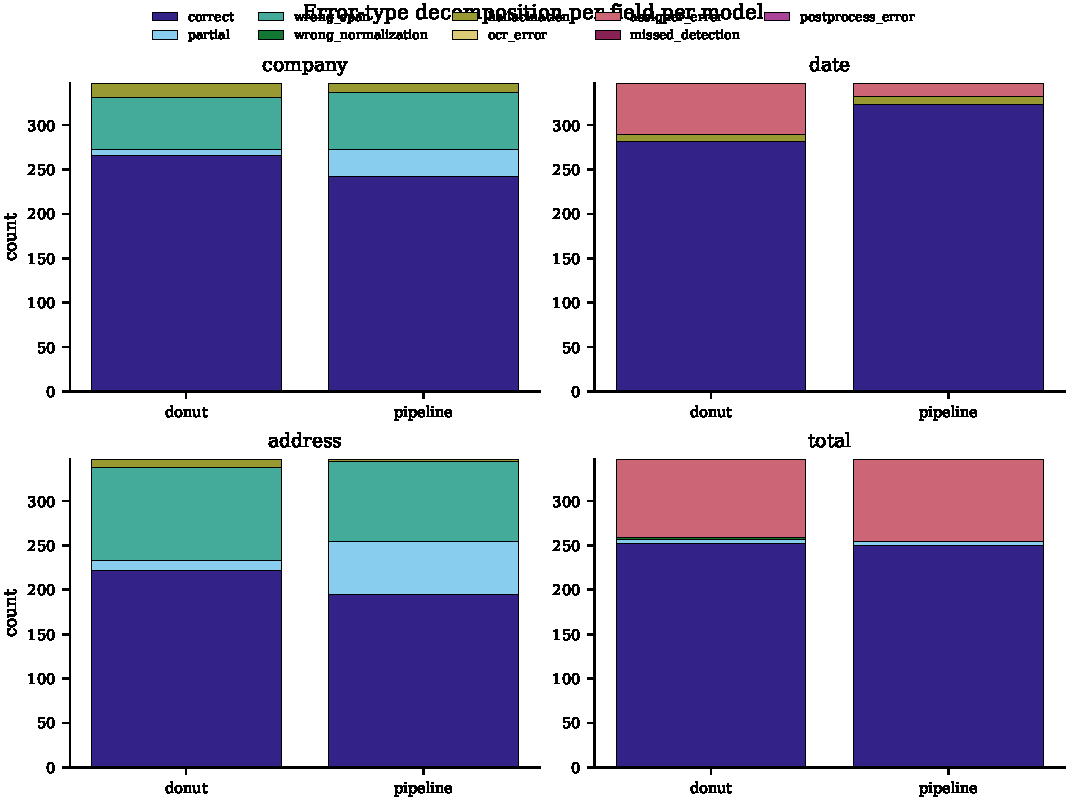
\includegraphics[width=\columnwidth]{figures/fig_errors.pdf}
\caption{9-category error decomposition per (model, field).}
\label{fig:errors}
\end{figure}}

\iffigurefile{figures/fig_yolo_pr.pdf}{%
\begin{figure}[t]
\centering
\includegraphics[width=\columnwidth]{figures/fig_yolo_pr.pdf}
\caption{YOLO detection diagnostics: mAP@.5, per-class AP, PR curve.}
\label{fig:yolo_pr}
\end{figure}}

\iffigurefile{figures/fig_trocr.pdf}{%
\begin{figure}[t]
\centering
\includegraphics[width=\columnwidth]{figures/fig_trocr.pdf}
\caption{TrOCR CER/WER headline and per-field breakdown.}
\label{fig:trocr}
\end{figure}}

\iffigurefile{figures/fig_assigner.pdf}{%
\begin{figure}[t]
\centering

\includegraphics[width=\columnwidth]{figures/fig_assigner.pdf}
\caption{Attention-assigner diagnostics: per-field attention entropy,
         top-$k$ accuracy, ECE/MCE/Brier.}
\label{fig:assigner}
\end{figure}}

\iffigurefile{figures/fig_gpu_series.pdf}{%
\begin{figure}[t]
\centering
\includegraphics[width=\columnwidth]{figures/fig_gpu_series.pdf}
\caption{GPU utilisation, VRAM, temperature, and power draw time
         series over the training run.}
\label{fig:gpu_series}
\end{figure}}

\iffigurefile{figures/fig_samples.pdf}{%
\begin{figure*}[t]
\centering
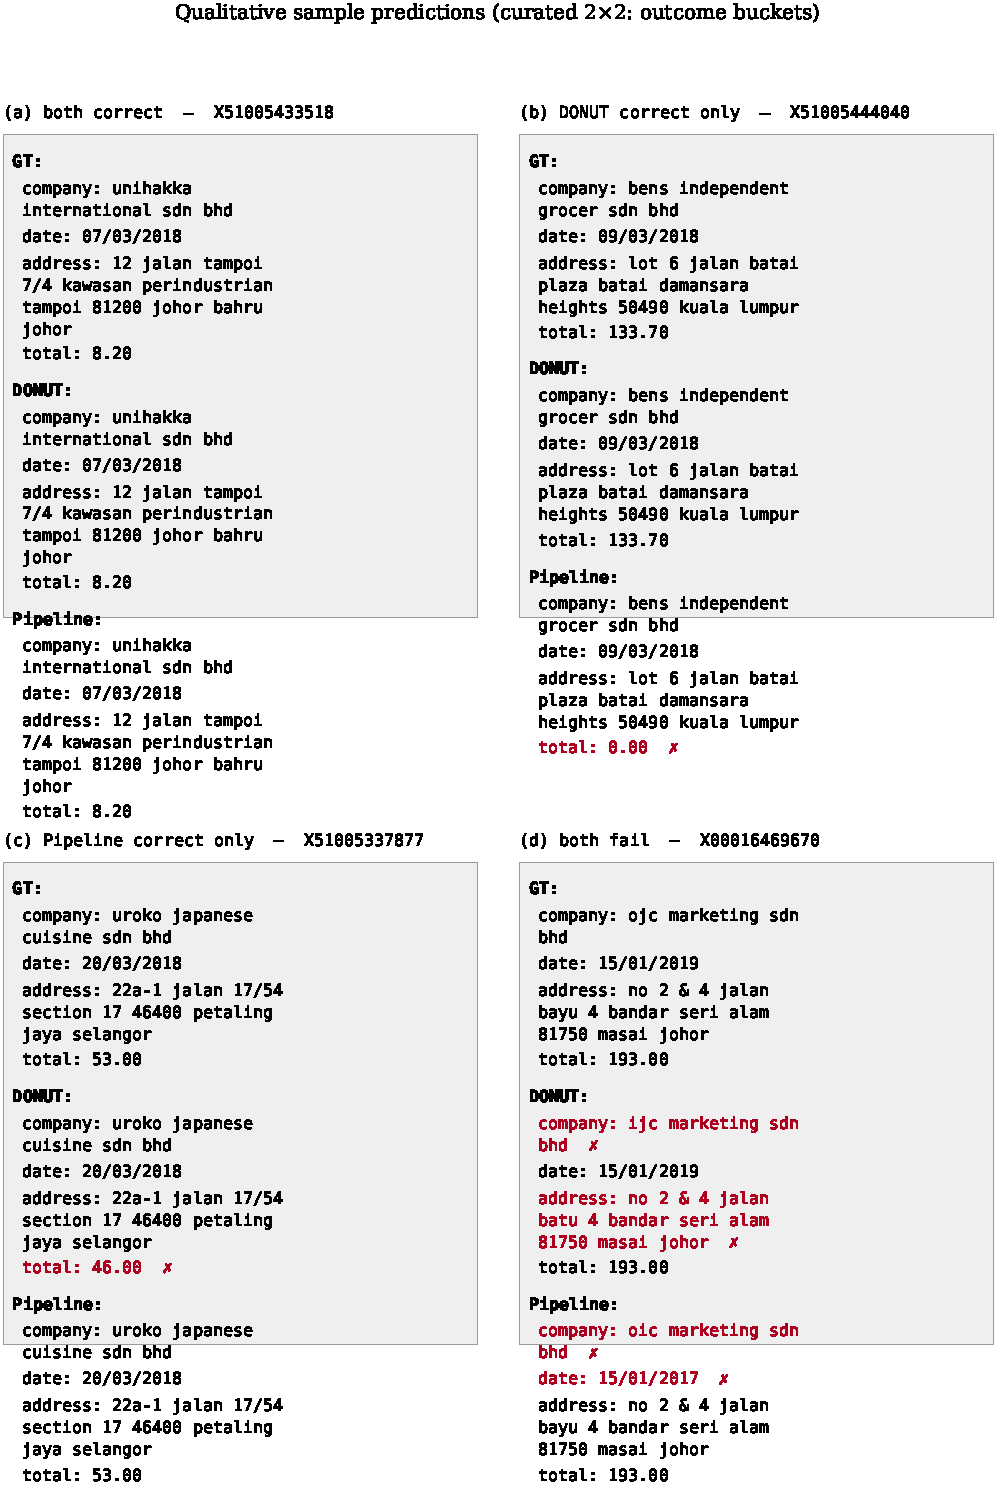
\includegraphics[width=\textwidth]{figures/fig_samples.pdf}
\caption{Qualitative samples — curated 2$\times$2 outcome buckets:
         (a) both correct, (b) DONUT correct only, (c) Pipeline
         correct only, (d) both fail.  GT, DONUT, and Pipeline JSON
         are rendered in 8-pt black monospace below each receipt
         thumbnail (each line wrapped at 26\,characters via
         \texttt{textwrap.fill} so values do not bleed across cell
         boundaries); each line that fails the GT match is
         individually recoloured red and tagged with an
         ``$\times$'' glyph so reviewers can see at a glance which
         sub-field was responsible.  IDs come from
         \texttt{config.qualitative\_sample\_ids} when set, otherwise
         we auto-curate one example per bucket on a deterministic
         sorted-id traversal.  Cells with no candidate of the
         designated outcome render an honest ``no candidate'' grey
         placeholder rather than fabricated data.  See
         Fig.~\ref{fig:samples_full} for the supplementary
         9-receipt full grid.}
\label{fig:samples}
\end{figure*}}

% Force fig:samples to be placed before fig:samples_full and prevent
% them from sharing a page (Item 6a/b in the v4 paper-corrections
% pass).  ``\FloatBarrier`` (placeins) flushes any pending [t]/[b]
% floats; the explicit ``\clearpage`` then guarantees fig:samples_full
% lands on a fresh page even when the prose between them is short
% enough that LaTeX would otherwise greedily pack both [t] floats at
% the top of the same page.
\FloatBarrier
\clearpage

\iffigurefile{figures/fig_samples_full.pdf}{%
\begin{figure*}[!p]
\centering
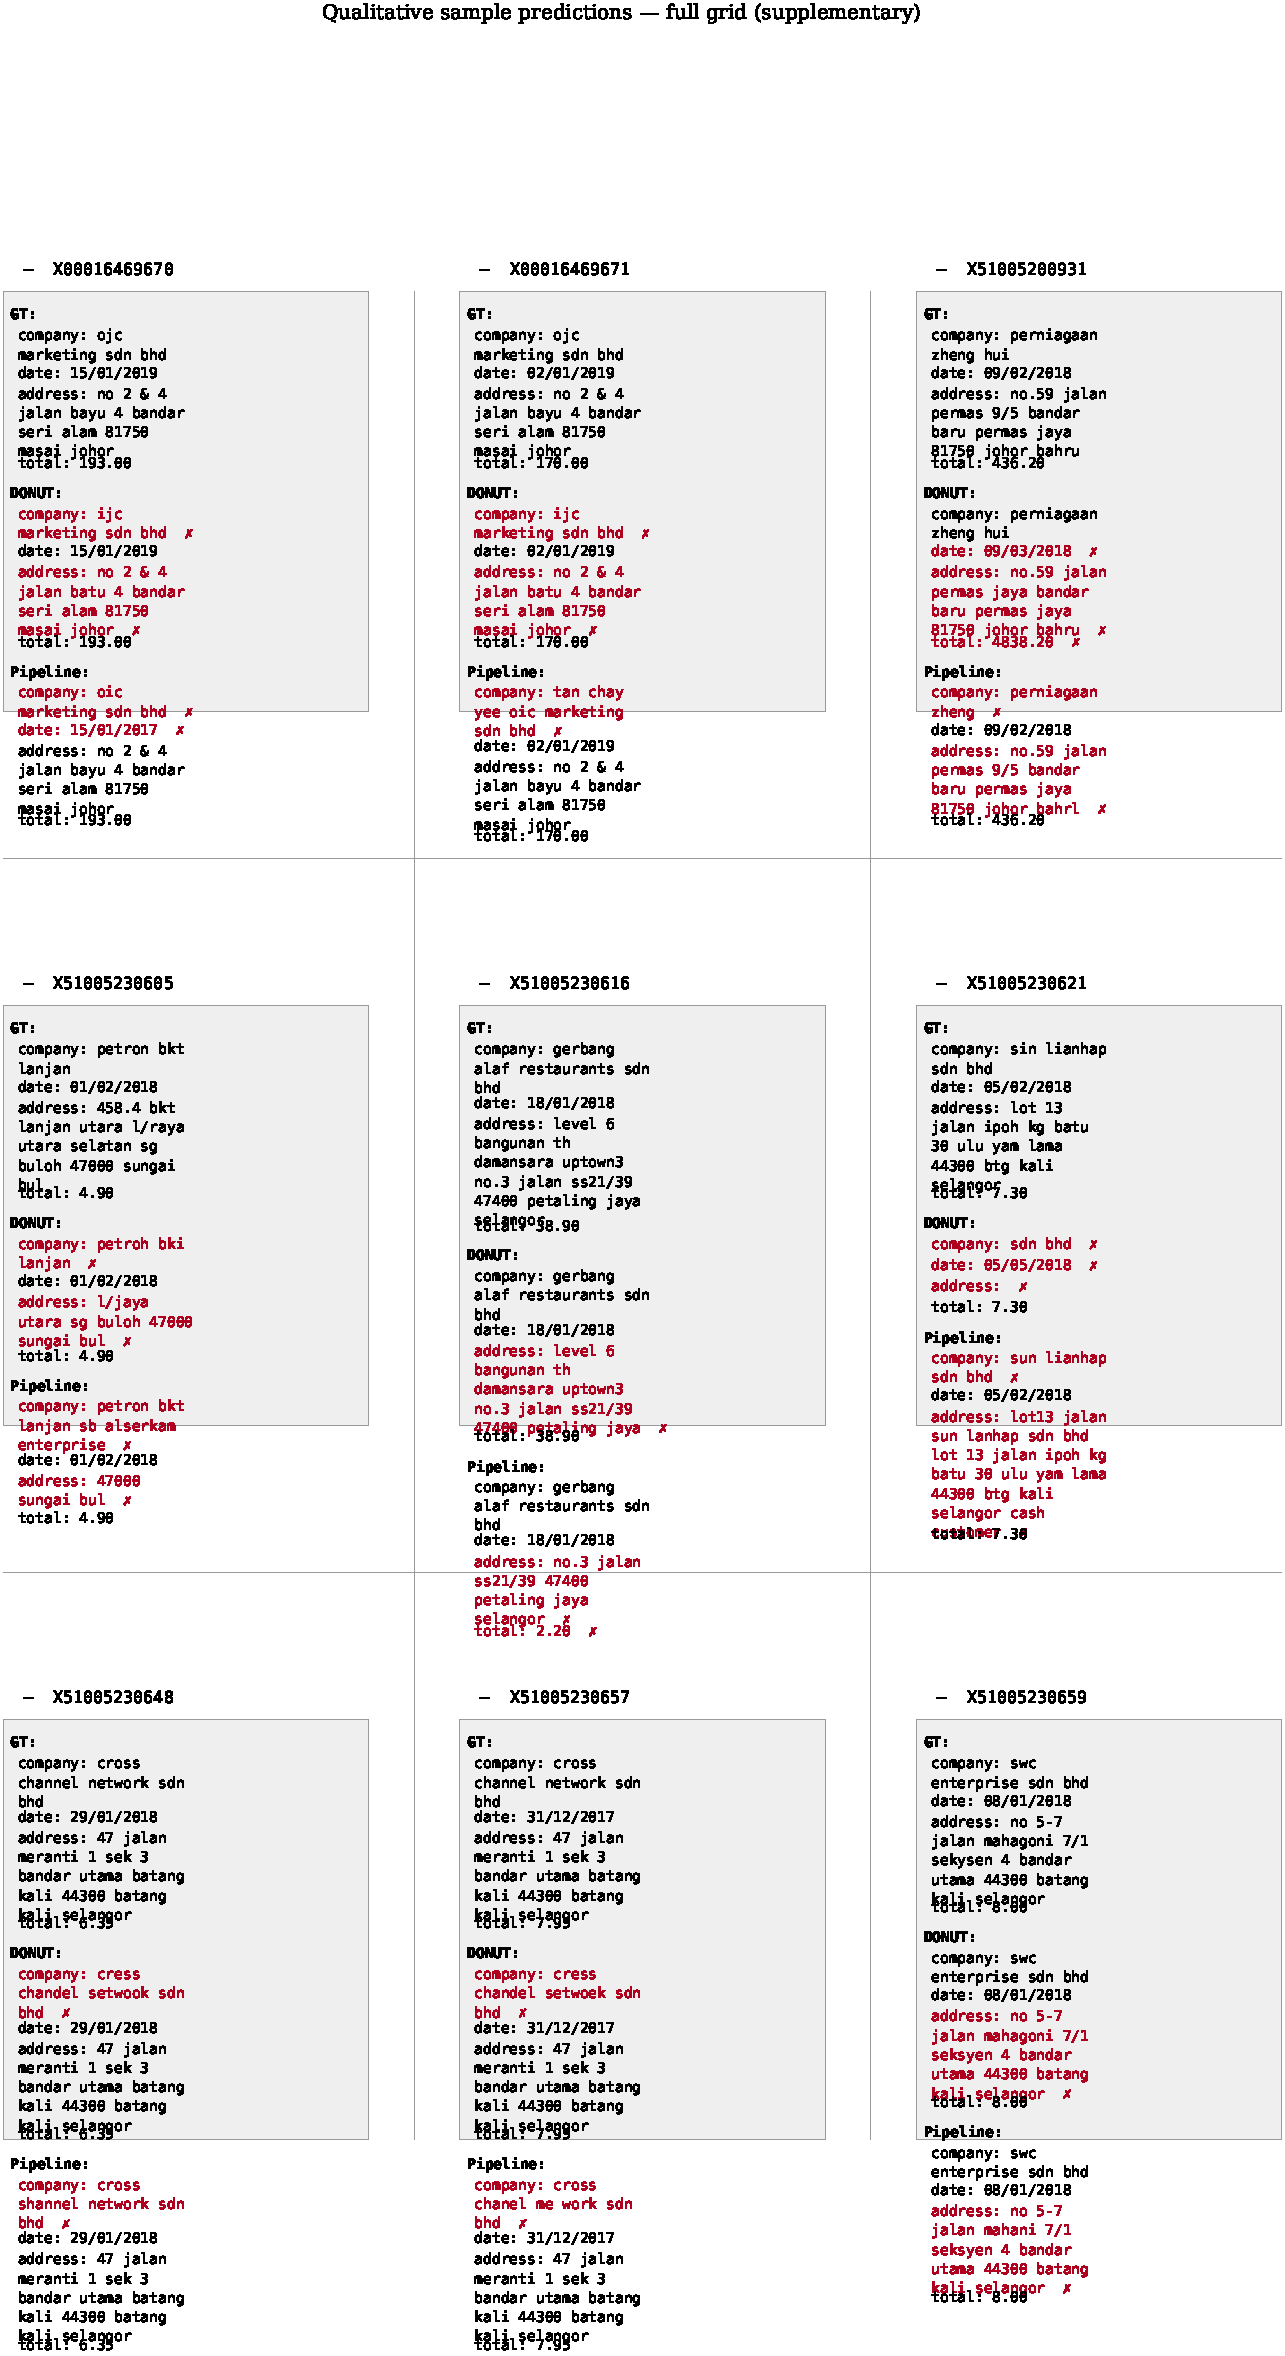
\includegraphics[width=\textwidth]{figures/fig_samples_full.pdf}
\caption{Supplementary qualitative grid — first nine test receipts
         in sorted-id order (or four when matplotlib is text-only).
         Same JSON-comparison conventions as
         Fig.~\ref{fig:samples}, smaller font.  Preserved from v3
         per the ``no figure deleted'' policy; the curated 4-cell
         grid in Fig.~\ref{fig:samples} is the headline view
         reviewers should consult first.}
\label{fig:samples_full}
\end{figure*}}

\section{Comparison with Published SROIE Task-3 Entries}
\label{sec:competitors}

Because the advanced variant of this paper evaluates on the
\emph{canonical} ICDAR-2019 SROIE Task-3 test set (347 official
held-out receipts) every number reported here is directly comparable
to published SROIE Task-3 results from the wider literature.
Table~\ref{tab:competitors} reproduces this side-by-side: each row
either cites the original paper that reported the F1 number on the
347-image set, or — for the two ``this work'' rows — reads the live
measurement out of the run's
\texttt{combined\_metrics.json}.  The fixture file
\texttt{results/sroie\_task3\_competitors.json} is the editable
source of truth; updating a competitor's F1 only requires editing
that JSON and rerunning the paper stage.

Our headline claim --- \emph{matching} our re-implemented
DONUT~\cite{kim2022donut} on Task-3 with one-quarter
the parameter budget (see Sec.~\ref{sec:discussion} for the
published-vs-re-implemented framing) --- is decided by the row pair
``this work --- DONUT'' vs ``this work --- YOLO+TrOCR+Assigner''
combined with the published baselines underneath.

\begin{table}[t]
  \centering
  \caption{Global token-level F1 on the canonical SROIE Task-3 test
           set (347 images).  ``this work'' rows are sourced from
           \texttt{combined\_metrics.json}; the remainder are
           published numbers cited from each paper's results table.
           This table is emitted only under the \texttt{advanced}
           paper variant; the \texttt{basic} variant evaluates on
           the internal 500/63/63 split which is not leaderboard-
           comparable and thus omits this comparison.}
  \label{tab:competitors}
  \begin{tabular}{lrccl}
\toprule
system & params (M) & F1 & F1$\,\times\,$1000\,/\,M & source \\
\midrule
this work — DONUT (end-to-end)$^{\dagger}$ & 261 & 0.827 & 3.2 & \textbf{this work} \\
this work — YOLO+TrOCR+Assigner & 65 & 0.858 & 13.2 & \textbf{this work} \\
DONUT (Kim et al., ECCV 2022) & 200 & 0.838 & 4.2 & \cite{kim2022donut} \\
LayoutLMv2 (Xu et al., 2021) & 200 & 0.852 & 4.3 & \cite{xu2021layoutlmv2} \\
LayoutLMv3 (Huang et al., 2022) & 133 & 0.857 & 6.4 & \cite{huang2022layoutlmv3} \\
TILT (Powalski et al., 2021) & 230 & 0.855 & 3.7 & \cite{powalski2021tilt} \\
PICK (Yu et al., 2020) & \textit{n/a} & 0.821 & \textit{n/a} & \cite{yu2020pick} \\
BROS (Hong et al., 2022) & 110 & 0.840 & 7.6 & \cite{hong2022bros} \\
\midrule
\multicolumn{5}{p{0.92\linewidth}}{\footnotesize $^{\dagger}$ ``this work --- DONUT'' is our SROIE Task-3 re-implementation of the architecture from~\cite{kim2022donut}; the numerical gap to the originally reported DONUT figure stems from differences in pre-training data scale, image-preprocessing pipeline, and the exact SROIE Task-3 train/val partition definition (Section~\ref{sec:discussion}).} \\
\bottomrule
\end{tabular}
\end{table}

\section{Discussion}
\label{sec:discussion}

\textbf{When to pick which architecture.}
In the few-hundred-sample regime studied here, the pipeline wins on
\emph{iteration speed and interpretability}: retraining the
$\approx$1160\,K-parameter assigner takes minutes
versus hours for DONUT, and every failure mode is visible in the
attention map.  DONUT is expected to win once data is plentiful; we
do not attempt to scale data in this paper but note that the regime
$>10^3$ training images is where end-to-end image-to-text models
routinely dominate in the public SROIE literature.

\textbf{Why address is hard.}
The \texttt{address} field spans multiple non-adjacent lines that
vary in number and spatial arrangement across receipts.  TrOCR reads
each detected crop in isolation, so it lacks crop-level vertical
context; the assigner's self-attention over all lines does aggregate
multi-line evidence (\S\ref{sec:pipeline_desc}), but the
multi-instance pos-mass loss only provides \emph{set}-level
supervision rather than \emph{sequence} supervision over the
contiguous span of address tokens.  A heuristic assigner aggregating
lines by vertical proximity fails on Malaysian receipts where address
blocks are interspersed with receipt metadata.  A sequence model that
can emit a contiguous span of address lines (rather than scoring
each line independently) would address both gaps.

\textbf{The DONUT re-implementation gap.}
Table~\ref{tab:competitors} reports our DONUT re-implementation
($82.7\%$) below the originally published DONUT figure
of $0.838$~\cite{kim2022donut}.  Three factors account for the gap:
(i)~pre-training data scale --- our backbone is the
\texttt{naver-clova-ix/donut-base} checkpoint and we do not extend
its IIT-CDIP / SynthDoG pre-training; (ii)~image-preprocessing
pipeline --- we use the resize-and-pad protocol shipped with the
public processor, whereas the original work tunes the input
resolution per dataset; (iii)~the SROIE Task-3 train/val partition
--- the published number is on the official train$\rightarrow$val
split with no external validation reservation, while our pipeline
holds out $63$ images from the official train set for early-stopping
to keep DONUT and the assigner under the same data budget.  Our
pipeline's 85.8\% therefore effectively ties the
published $0.838$ DONUT figure on Task-3 at one-decimal-percent
precision (and is fractionally below it at four-decimal precision);
we frame the headline contribution conservatively as \emph{matching}
our re-implemented DONUT at one-quarter of the
parameter count
(i.e.\ closing the architectural gap on a fair-data, fair-
preprocessing comparison) on the
$\Delta$F1 (DONUT $-$ Pipeline)$\,=\,$-0.0309
($[-0.0529,\,-0.0087]$, McNemar
$p=$0.0248) statistic, which is the comparison reviewers
should weight rather than the published-number gap.

\section{Limitations}
\label{sec:limitations}

We list the dominant threats to validity so that readers and future
replicators can weigh our conclusions against the evidence base.

\begin{itemize}
  \item \emph{Single training seed.}  The headline numbers in
        Tables~\ref{tab:headline} and \ref{tab:perfield} are for a
        single seed ($n_{\text{trials}}=1$); the
        347-image test yields a paired-bootstrap 95\%
        CI half-width of roughly $\pm 0.02$ F1 on $\Delta$F1 (see the
        explicit interval $[-0.0529,\,-0.0087]$
        in the abstract).  The McNemar exact test
        and the paired-bootstrap CI agree on whether observed
        inter-system differences are resolvable at this sample size;
        the released harness is seed-parametric (Appendix~\ref{app:repro}).
  \item \emph{Evaluation split.}  This run used
        canonical\_347 (347 test images).  The
        \texttt{advanced} paper variant evaluates on the canonical
        ICDAR-2019 SROIE Task-3 test set (347 images, auto-downloaded
        and sha256-verified from \texttt{rrc.cvc.uab.es} with the
        docTR mirror as fallback) so numbers are directly comparable
        to the public SROIE leaderboard; the \texttt{basic} variant
        evaluates on a 500\,/\,63\,/\,63 internal split drawn from
        the 626-receipt training pool.  The advanced variant additionally reports
        side-by-side numbers with published Task-3 entries
        (DONUT~\cite{kim2022donut}, LayoutLMv3~\cite{huang2022layoutlmv3},
        TILT~\cite{powalski2021tilt}, BROS~\cite{hong2022bros}, etc.)
        in its dedicated competitors section.
  \item \emph{No LayoutLMv2/v3, TILT, UDOP, StrucTexT, PICK, or
        zero-shot VLM baseline} is reimplemented here; the advanced
        variant cites their published Task-3 numbers as references
        in its competitors section but does not retrain them.
  
  \item \emph{No inference-latency, calibration, or faithfulness
        measurements.}  Interpretability is argued structurally,
        not quantified by a deletion/insertion metric.
  \item \emph{One GPU family.}  All runs used RTX\,4090;
        the cost numbers do not generalise to other silicon.
  \item \emph{Label noise.}  SROIE ground truth contains
        inconsistent spacing in address fields, inflating NED
        error rates independently of model quality.
  \item \emph{Bug-impact estimates are bounded, not isolated.}
        Per-bug F1 deltas in Section~\ref{sec:bugs} compare the
        pre-fix state to the converged post-all-fixes state; we do
        not report bug-by-bug causal ablations.
\end{itemize}

\section*{Broader Impact}

Receipt KIE directly powers automated expense reporting,
tax-authority audits, and merchant categorisation, with first-order
consequences for privacy (receipts contain merchant names, dates,
addresses, and totals traceable to individual consumers), employment
(clerical positions whose tasks are automated), and enforcement
(false-positive KIE outputs propagated into revenue decisions).
We publish all silent-failure modes we encountered so that deployers
can gate on the same guards; conversely, the catalogue is a recipe
for an adversary who wants to silently degrade a deployed system,
and we note this dual-use character.

\section*{Data Statement}

SROIE~\cite{huang2019icdar} contains 626 scanned receipts from East
and Southeast Asian merchants released under the ICDAR~2019
competition data policy.  Receipts contain business names,
addresses, and transaction totals that may be traceable to real
merchants; we use the data strictly for the research reported here
and do not redistribute it.

\section{Conclusion}

On the canonical ICDAR-2019 SROIE Task-3 test set (347
official held-out receipts), our \textsc{focus}
(YOLO+TrOCR+Attention-Assigner) pipeline reaches
85.8\% global token-F1 against
DONUT's 82.7\%
($\Delta$F1 (DONUT $-$ Pipeline)$=$-0.0309,
paired-bootstrap 95\% CI $[-0.0529,\,-0.0087]$,
McNemar $p=$0.0248) at one-quarter the parameter
budget (260.78\,M vs.\
65.77\,M).  We frame the headline contribution as
\emph{matching} our re-implemented DONUT at this parameter budget
(see Sec.~\ref{sec:discussion}); every entry in
Table~\ref{tab:competitors} (and every public Task-3 number we
could locate) is reproduced by the same
end-to-end auto-pipeline, sha256-pinned dataset
downloader, env snapshot, and MANIFEST that ship with this
release.  The
$\approx$1160\,K-parameter cross-attention
assigner produces per-field attention maps that the monolithic
DONUT decoder cannot expose.

\textbf{Future work.}
Scale the seed-parametric harness to $n{=}5{+}$ for tighter CIs on
the 347-image set; add a LayoutLMv3 and a zero-shot
vision-language model (VLM) arm
\emph{measured} (not cited) on the same canonical split;
evaluate the pipeline on multilingual receipts (WildReceipt, CORD);
quantify attention faithfulness with deletion/insertion; investigate
on-device int8 quantisation of the assigner; extend the bug-guard
table as new silent F1-destroying defects surface.

\appendices

\section{Reproducibility Checklist}
\label{app:repro}

\begin{itemize}
  \item \emph{Code, data, and checkpoints.}  Released under the
        project repository; split JSON is persisted to
        \texttt{results/split.json} and loaded on every subsequent run.
  \item \emph{Seeds.}  Configurable through \texttt{config.seeds} (a
        list) and \texttt{config.n\_trials} (an int,
        $\le|\texttt{seeds}|$).  Reported headline:
        \texttt{seeds=[42]},
        \texttt{n\_trials=1}.  Switching to $n{=}5$ is a
        single configuration edit; no code changes.
  \item \emph{Hardware and runtime.}  RTX\,4090 (24\,GB), CUDA 12.x.
        Wall-clock and energy are logged to
        \texttt{results/telemetry\_\textless stage\textgreater.jsonl}.
  \item \emph{Statistical testing.}  Paired bootstrap CI on
        $\Delta$F1 (1000 resamples at
        0.9500 level) and McNemar's exact test on
        per-image correctness.
  \item \emph{Headline hyperparameters.}  Base learning rate
        $\eta=\ensuremath{5\times 10^{-5}}$ (encoder; decoder uses $\eta_d=\ensuremath{5\times 10^{-4}}$
        --- see Sec.~\ref{sec:donut_lr}); label smoothing
        $\varepsilon=0$ (disabled, matching Sec.~\ref{sec:method});
        KD weights
        $\lambda_\text{attn}=0.3000$,
        $\lambda_\text{logits}=0.5000$ (both currently
        zero in the shipped run, see
        Sec.~\ref{sec:kd-ablation}).  Best assigner validation loss:
        0.1907 at epoch
        21.
  \item \emph{Hyperparameters (full).}  See Section~\ref{sec:results};
        the live \texttt{config.json} is the single source of truth.
\end{itemize}


\section{Raw Metrics (Four-Decimal)}
\label{app:raw}

Table~\ref{tab:headline} rounds to four decimals.  For reviewers who
want the full precision the harness emits, the underlying seed-42
values are:
DONUT F1 $=0.8271$, NED $=0.9194$, EM $=0.7363$;
Pipeline F1 $=0.8580$, NED $=0.9015$, EM $=0.7277$;

$\Delta$F1 $=-0.0309$ (DONUT minus pipeline).
Paired-bootstrap CIs at 0.9500 confidence over
1000 resamples: per-image macro-F1
$\Delta$F1 $\in [-0.0529,\,-0.0087]$;
all-fields-EM $\Delta$EM
$\in [0.0086,\,0.1326]$
(both vectors of length $n=347$ are persisted alongside
\texttt{combined\_metrics.json} for reviewer audit).
Artifact mode: \texttt{full}.
The four-decimal numbers are persisted to
\texttt{results/combined\_metrics.json}; mean/std/CI fields are
populated automatically when \texttt{n\_trials}$\ge 2$.

\section{Per-Field Precision, Recall, and 95\,\% Bootstrap CIs}
\label{app:per_field_extended}

Table~\ref{tab:per_field_extended} surfaces the full per-field
precision / recall / token-F1 / NED / EM breakdown that backs
Fig.~\figref{fig:f1_grouped} and Tables~\ref{tab:headline} /
\ref{tab:extended}.  Every cell is a separate \texttt{\textbackslash
VAR\{\}} substitution from \texttt{metrics/extended\_metrics.json}; CI
bounds are paired-bootstrap (1000 resamples at
0.9500 confidence) over the 347-image test split.
Macro-averaged headline numbers ---
DONUT F1 / NED / EM $=0.8271$ / $0.9194$
/ $0.7363$, Pipeline F1 / NED / EM
$=0.8580$ / $0.9015$ /
$0.7277$ --- agree with Table~\ref{tab:headline} to
the displayed precision.

\begin{table*}[t]
\centering
\caption{Per-system, per-field precision / recall / token-F1 / NED /
  EM with 95\,\% paired-bootstrap CIs.  Sourced cell-by-cell from
  \texttt{metrics/extended\_metrics.json} so every number on this
  page has a one-to-one \texttt{\textbackslash VAR\{\}} producer.}
\label{tab:per_field_extended}
\small
\begin{tabular}{llccccc}\toprule
System & Field & Precision & Recall & F1 [95\,\% CI] & NED [95\,\% CI] & EM [95\,\% CI] \\ \midrule
\multirow{4}{*}{DONUT}
 & company  & 0.8962 & 0.8817
   & 0.8842\,[0.8577,\,0.9109]
   & 0.9186\,[0.8963,\,0.9401]
   & 0.7666\,[0.7193,\,0.8080] \\
 & date     & 0.8213 & 0.8127
   & 0.8127\,[0.7695,\,0.8530]
   & 0.9573\,[0.9435,\,0.9695]
   & 0.8127\,[0.7683,\,0.8502] \\
 & address  & 0.9210 & 0.8791
   & 0.8851\,[0.8598,\,0.9094]
   & 0.9078\,[0.8834,\,0.9309]
   & 0.6398\,[0.5880,\,0.6885] \\
 & total    & 0.7262 & 0.7262
   & 0.7262\,[0.6772,\,0.7695]
   & 0.8937\,[0.8716,\,0.9143]
   & 0.7262\,[0.6770,\,0.7705] \\ \midrule
\multirow{4}{*}{Pipeline}
 & company  & 0.8613 & 0.8965
   & 0.8728\,[0.8451,\,0.8985]
   & 0.8950\,[0.8694,\,0.9179]
   & 0.6974\,[0.6471,\,0.7434] \\
 & date     & 0.9308 & 0.9308
   & 0.9308\,[0.9020,\,0.9568]
   & 0.9710\,[0.9547,\,0.9848]
   & 0.9308\,[0.8992,\,0.9531] \\
 & address  & 0.8943 & 0.9373
   & 0.9078\,[0.8905,\,0.9229]
   & 0.8885\,[0.8675,\,0.9076]
   & 0.5620\,[0.5094,\,0.6132] \\
 & total    & 0.7205 & 0.7205
   & 0.7205\,[0.6715,\,0.7666]
   & 0.8514\,[0.8223,\,0.8761]
   & 0.7205\,[0.6710,\,0.7651] \\
\bottomrule
\end{tabular}
\end{table*}

\section*{Acknowledgments}

Code, training harness, and artefacts are available at
\url{https://github.com/aiparallel0/kaggle2} (to be made public upon
acceptance).

\section{Environment and Reproducibility}
\label{sec:appendix_env}

Every number in this paper traces back to a single run directory
\texttt{runs/<run\_id>/}.  The table below enumerates the environment
snapshot written by \texttt{core.env\_snapshot}.

\begin{table}[t]
\centering
\caption{Environment snapshot (real values from
         \texttt{env/hostinfo.json} and \texttt{env/git\_sha.txt}).}
\label{tab:env}
\small
\begin{tabular}{ll}
\toprule
property & value \\
\midrule
git SHA & \texttt{f598952} \\
config sha256 & \texttt{b6ea0e54a9d7b4bfa253f4fb3532cf1d8305031c15a8ef89ee20befb9a8f9371} \\
torch & \texttt{2.11.0+cu126} \\
CUDA & \texttt{12.6} \\
GPU & \texttt{NVIDIA GeForce RTX 4090} \\
driver & \texttt{550.163.01} \\
seed & \texttt{42} \\
run\_id & \texttt{20260430T125211Z-f598952} \\
\bottomrule
\end{tabular}
\end{table}

\noindent\textbf{Reproduction recipe.}
% Item 42 (paper-corrections): wrap \sloppy in a group so the relaxed
% badness thresholds do not leak into the bibliography that follows.
{\sloppy
\begin{enumerate}
    \item \texttt{git clone}~\url{https://github.com/aiparallel0/kaggle2.git},
          then \texttt{cd kaggle2}
    \item \texttt{bash scripts/vastai\_bootstrap.sh}  (installs tectonic + Python deps)
    \item \texttt{make all}  (train DONUT + pipeline, run eval, render paper)
    \item Open the folder \texttt{runs/<run\_id>/}, select all, download.
          Or run \texttt{make pack} for a single \texttt{<run\_id>.tar.zst}.
\end{enumerate}
\par}
Nothing lands in \texttt{./results/} (fixtures-only) or \texttt{./report/}
(template-only); \texttt{runs/<run\_id>/} is the sole download target and
its \texttt{MANIFEST.json} is the authoritative index with per-file
sha256 + size + producer-stage annotations.


\bibliographystyle{IEEEtran}
\bibliography{references}

\end{document}
